% Autor: Lukas Deeken
% Letzte Bearbeitung: 01.05.2022

\chapter{Elektrische Systeme}
\FloatBarrier
\section{Akkumulator}
Im Akkumulator befinden sich neben den Zellen in Ihren Zellstacks und dem \acfirst{AMS} auch diverse andere Systeme die zum Betrieb des Fahrzeuges essentiell sind. Diese Systeme werden im folgenden Kapitel erläutert. Die Abbildung \ref{fig:accumulator-layout} gibt eine Übersicht wo sich diese Systeme befinden und wie sie zusammenhängen.

\begin{figure}
	\centering
	\includegraphics[width=1\linewidth]{"bilder/Accumulator Layout"}
	\caption{Akkumulator Layout}
	\label{fig:accumulator-layout}
\end{figure}

\FloatBarrier
\subsection{\ac{AMS} Master und Slave}
In diesem Kapitel werden die Subsysteme des \ac{AMS} näher betrachtet.
\FloatBarrier

\subsubsection{Precharge}
Der Precharge verhindert einen Funkenschlag und damit das Verschweißen der \acfirst{AIR}`s beim Schließen. Dies wird erreicht indem der Zwischenkreis bereits vor dem Durchschalten der \ac{AIR}`s auf die Akkuspannung aufgeladen wird. Anhand des Blockschaltbildes \ref{fig:precharge-blockschaltbild} lassen sich die einzelnen funktionellen Blöcke herausarbeiten.

\begin{figure}
	\centering
	\includegraphics[width=0.6\linewidth]{"bilder/Precharge Blockschaltbild"}
	\caption{Blockschaltbild Precharge}
	\label{fig:precharge-blockschaltbild}
\end{figure}

Kernelement ist die Verbindung der positiven Seite des Zwischenkreises mit der positiven Seite des Akkumulators über ein mechanisches Relais, und die Überwachung selbigens. Diese kann nicht mit einer \acfirst{AUX} Beschaltung umgesetzt werden, da Relais in diesem Leistungsbereich \acfirst{idR} nicht mit derartigen Funktionen ausgerüstet sind. Eine Besonderheit bei dem gewählten Relais ist die geringe Baugröße, aber auch ein damit einhergehendes niedriges Stromrating, so das der Einschaltstrom des Relais sehr klein gehalten werden muss. Aus diesem Grunde bedarf es einer Stromquelle welche zu beginn einen niedrigen Strom liefert, und diesen dann nach dem erfolgten Schalten anhebt. Nun zur Klärung der einzelnen funktionellen Gruppen und der Schaltzustände.

\begin{figure}
	\centering
	\includegraphics[width=1\linewidth]{"bilder/Precharge Blockschaltbild Detail"}
	\caption{Detail Schaltplan Precharge}
	\label{fig:precharge-blockschaltbild-detail}
\end{figure}

Der Precharge schaltet durch sobald SC\textsubscript{end} high wird. Dies führt zum Durchschalten des Relais. Nun fließt ein Strom über M1 zum Relais, bei der Verschaltung von M1 und R54 handelt es sich um eine Konstantstromquelle welche \ensuremath{0,05A} liefert. Wie diese Art von Schaltung im Detail funktioniert ist unter \ref{sec: TSAL Logik Discharge} näher erläutert. Parallel fließt ein Strom über U3 zu C58 und lädt diesen. Nach kurzer Zeit führt dies dazu das Q10 durchschaltet, nun wird der Strom durch den Widerstand der \acfirst{PTC}-Elemente begrenzt so das der Strom auf ca. \ensuremath{0,6 A} ansteigen kann. Die Überwachung erfolgt indem mithilfe eines DC Wandlers die Akkuspannung um \ensuremath{24 V} angehoben wird und diese über einen Optokoppler auf das Precharge Relais gelegt wird. Sobald das Relais geschlossen ist fließt somit ein Strom über U22 sodass bei PCHRG\textsubscript{ACT} eine Spannung anliegt.\\
\\
Im Ausschaltmoment wird das Relais durch die Kapazität C12 für kurze Zeit offen gehalten sodass zuerst der Mosfet Q10 abschaltet und so die Schaltleistung im Relais minimiert wird.
\FloatBarrier

\subsubsection{\ac{AIR} Detection}

\begin{figure}
	\centering
	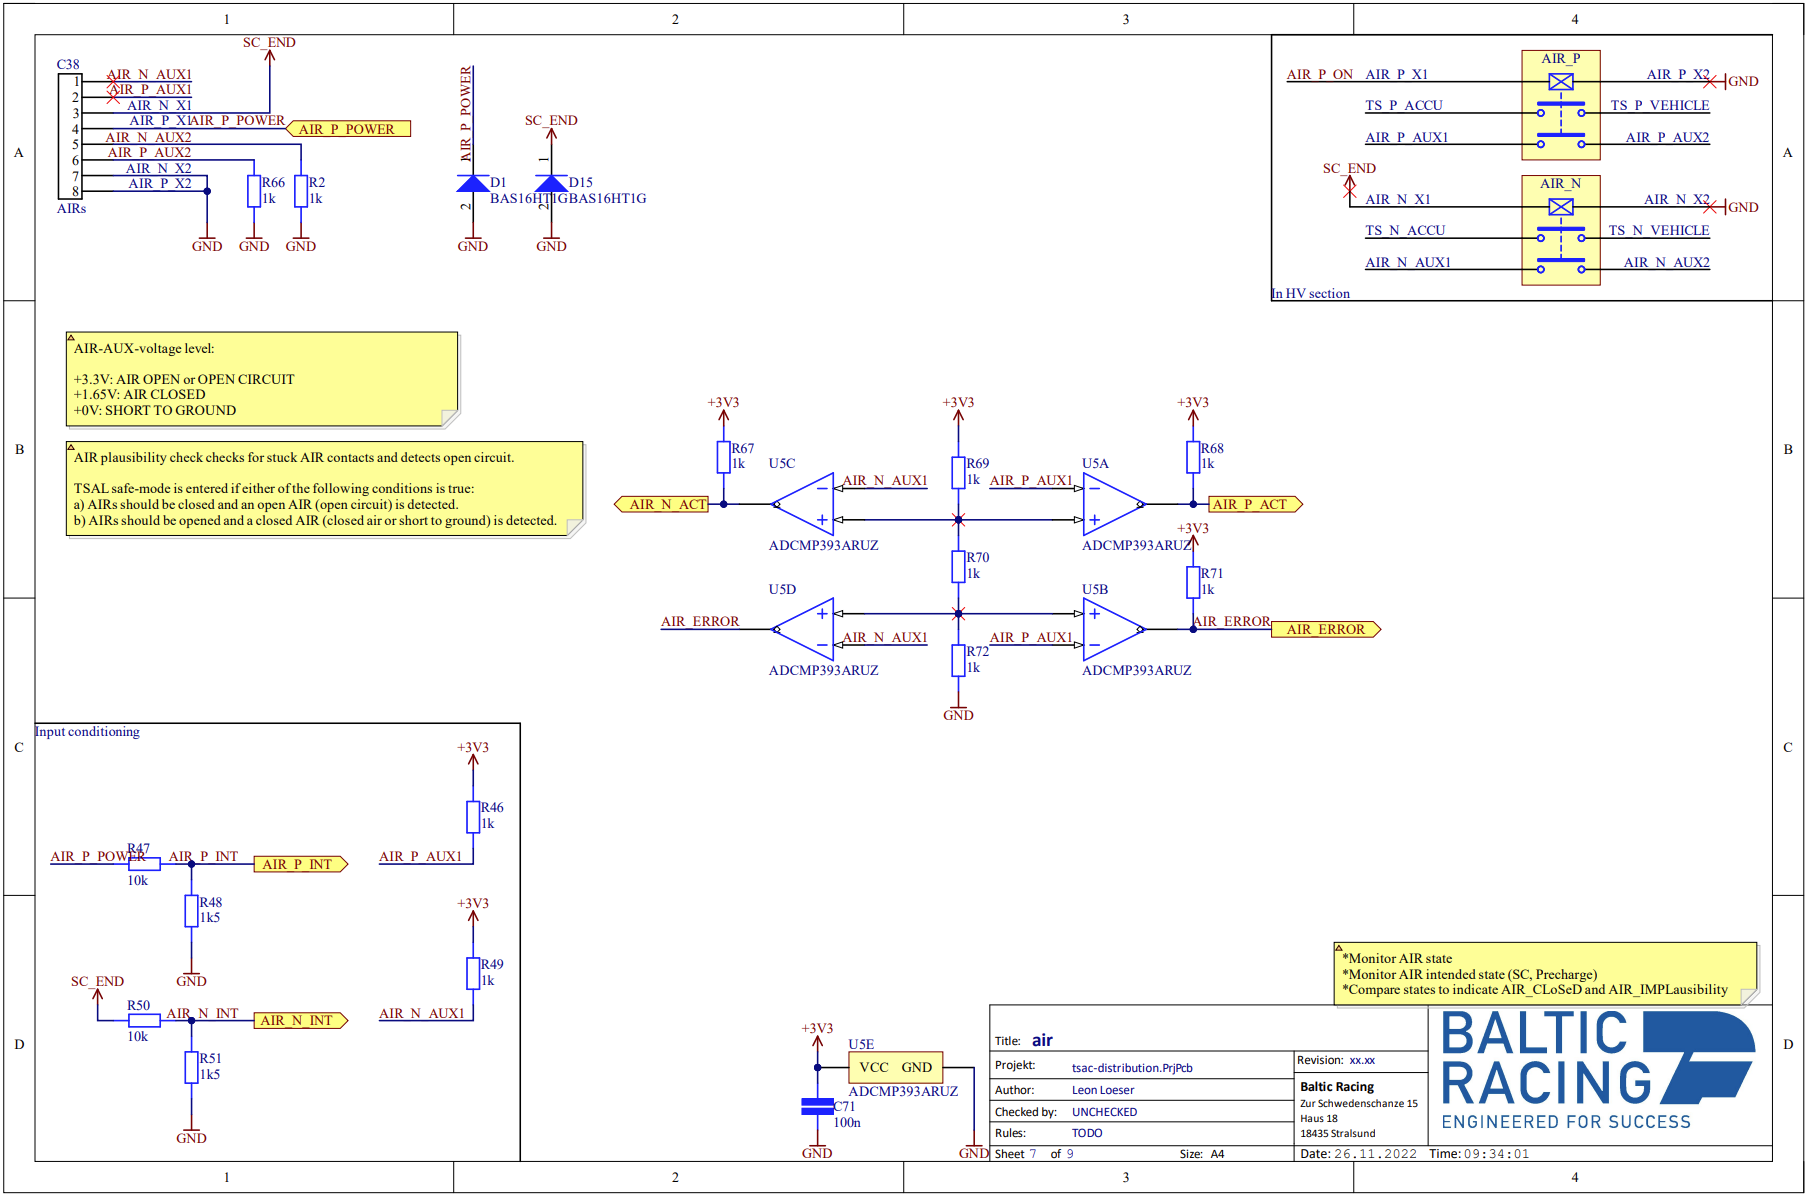
\includegraphics[width=0.8\linewidth]{bilder/AIR_conditioning}
	\caption{Schaltplan AIR}
	\label{fig:airconditioning}
\end{figure}

Sinn der \ac{AIR} Detection ist es die Signale von den \ac{AIR}`s in Sinnvolle Logikpegel umzusetzen welche im späteren Verlauf weiter verwendet werden können. Oben rechts auf dem Schaltplan sind die \ac{AIR}`s dargestellt. Relevant sind dabei die X-Signale welche den Schaltzustand des Relais kontrollieren und die \ac{AUX}-Signale welche den Schaltzustand überwachen. Die \ac{AUX} Signale werden mit \ensuremath{3,3V} über einen Gleichwertigen \ensuremath{1 k\Omega} Spannungsteiler versorgt, so das bei geöffnetem Relais die \ensuremath{3,3V} an \ac{AUX} 1 anliegen, bei geschlossenem Relais durch den Spannungsteiler \ensuremath{1,65V} und bei einem Kurzschluss in der Signalleitung zu Masse \ensuremath{0V} anliegen. Diese Spannungspegel werden jetzt in einer Komparatorschaltung verglichen. Die beiden oberen Komparatoren geben ein High-Signal aus wenn die Spannung an den \ac{AUX} Kontakten kleiner ist als die Referenzspannung und damit die Relais geschlossen oder auf Masse kurzgeschlossen sind. Die beiden unteren Komparatoren geben ein Low-Signal aus wenn die Spannung größer ist als die Referenzspannung und damit das Relais geschlossen oder geöffnet ist. Sofern also der tatsächliche Zustand des Relais high ist und der Fehler low kann zum Beispiel geschlussfolgert werden das jenes Relais geschlossen ist.
\FloatBarrier
\subsubsection{\ac{AMS}}
Das eigentliche Batteriemanagement wird von vom LTC 6804 übernommen. Hierbei handelt es sich um einen \acfirst{IC} welcher speziell für die Aufgabe des Batteriemanagments von Linear Technology entwickelt wurde. Relevante Aufgaben dieses Chips ist die differentielle Messung der Zellspannungen im Stack. Weiter übernimmt der \ac{IC} die Temperaturmessung über 5 frei nutzbare \acfirst{GPIO}`s welche auch \acfirst{ADC} Funktionalität unterstützen. Z u guter Letzt wird der Chip als Treiber für Mosfets benutzt welche die Zelle auf den Balancingwiderstand schalten. Die notwendige Kommunikation erfolgt über einen proprietären 2 drahtigen linearen isolierten \acfirst{SPI} Bus. Jeder Chip hat dabei 4 Adressbits zur Konfigurierung. Das Kommunikationsinterface zischen dem \acfirst{Iso}-\ac{SPI}- und dem \ac{SPI}-/Bus des Mikrocontroller erfolgt über den LTC 6820 welcher für exakt diese Aufgabe entwickelt wurde. Mit den 5 Eingängen am Chip sind nun 11 verschiedene \acfirst{NTC}`s auszuwerten, dies geschieht mit Hilfe eines Demuxers und eines Invertierers.
\begin{figure}
	\centering
	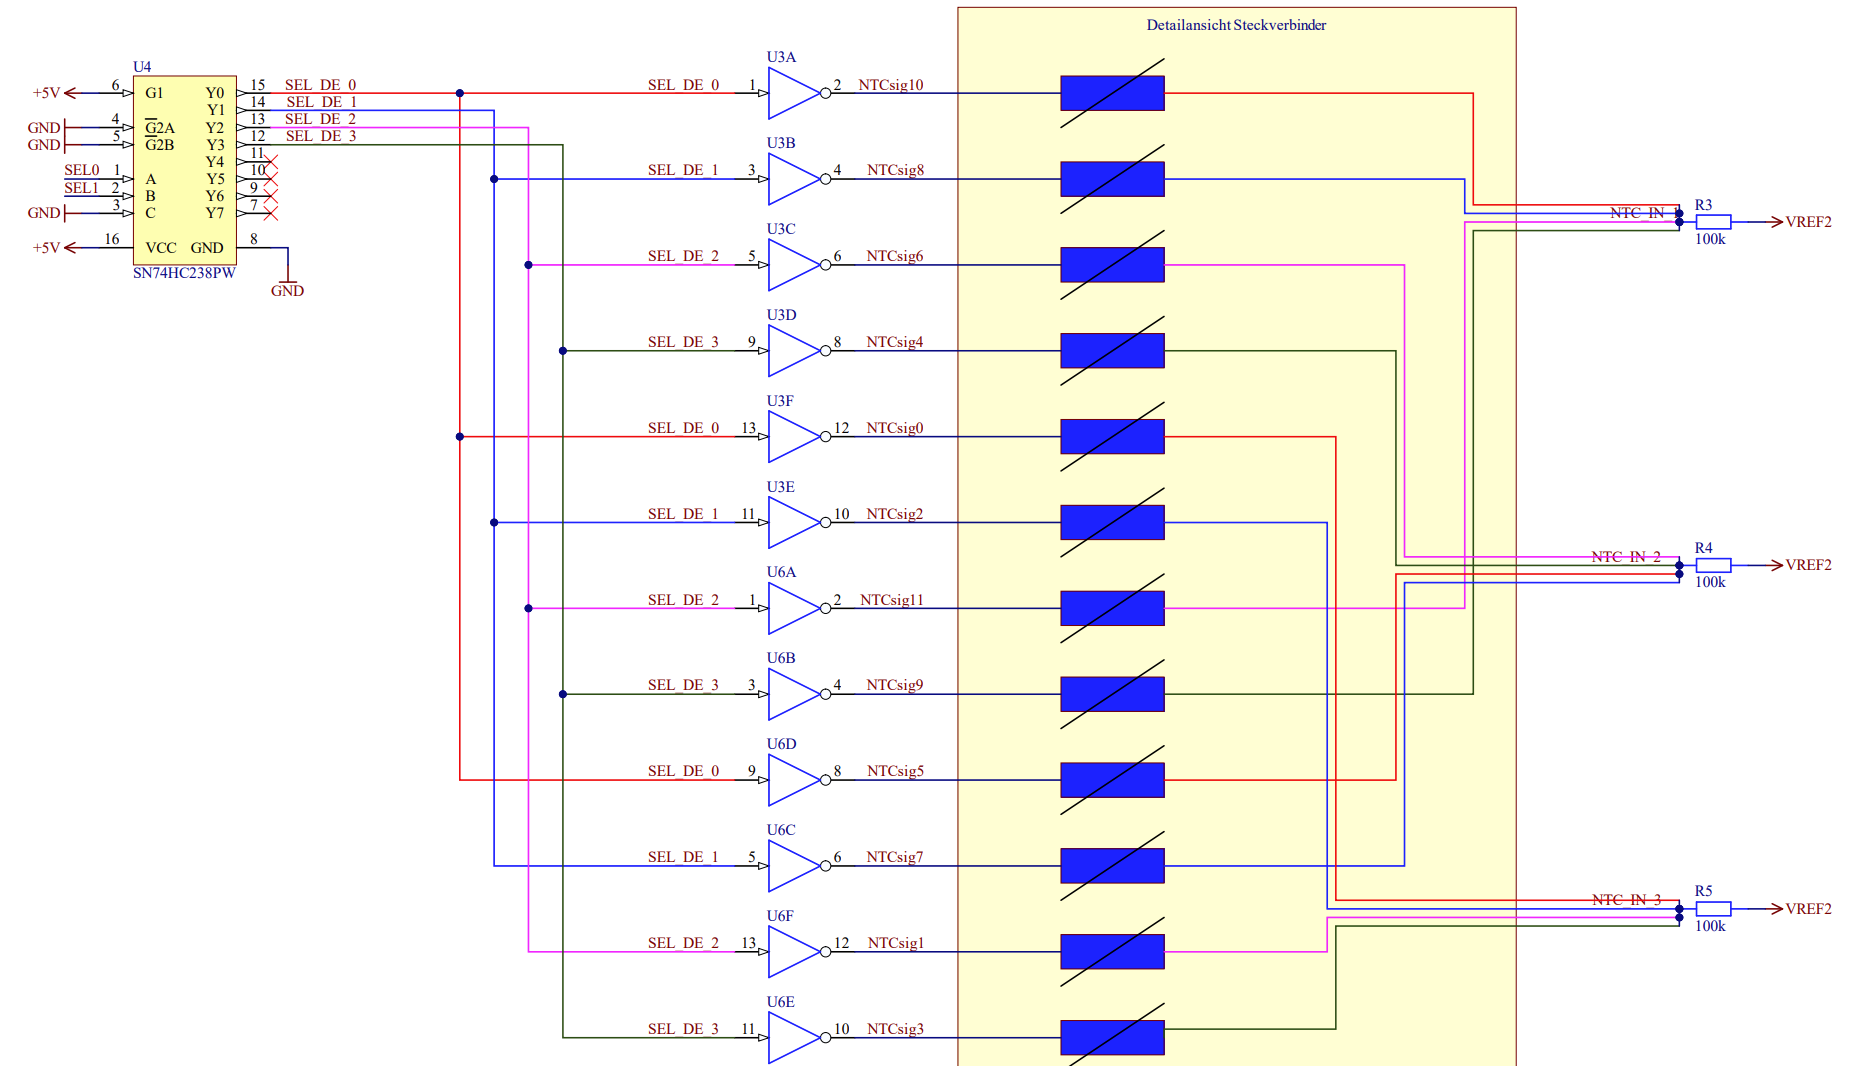
\includegraphics[width=0.7\linewidth]{bilder/AMS_NTC_Measurement}
	\caption{Schaltplan \ac{AMS}-\ac{NTC}-Messung}
	\label{fig:amsntcmeasurement}
\end{figure}

Zum Verständnis der Logik ist in der Abbildung \ref{fig:amsntcmeasurement} der Signalablauf dargestellt. Dieser wird nun einmal beispielhaft durchlaufen. Die Bits SEL\textsubscript{0} und SEL\textsubscript{1}, in diesem Beispiel low und high, vom LTC 6804 (U1) gehen auf die Eingänge A und B am Demuxer (U6). G2\textsubscript{A} und G2\textsubscript{B} sind immer auf low gesetzt und G1 immer auf high. Mit der Tabelle \ref{Demuxer_Logiktabelle} aus dem Datenblatt wird nun der Ausgang von Y\textsubscript{0} bis Y\textsubscript{3} bestimmt.

\begin{figure}
	\centering
	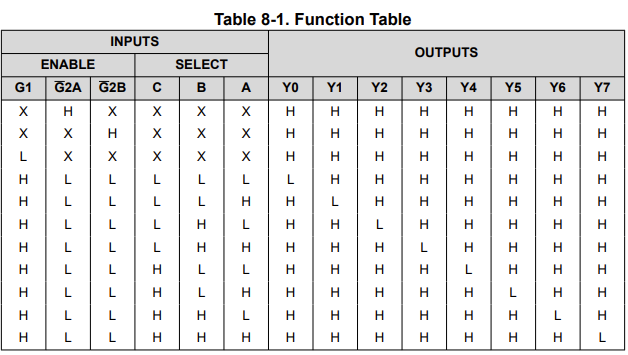
\includegraphics[width=0.5\linewidth]{bilder/AMS_demuxer_logiktabelle}
	\caption{Logiktabelle Demux \cite{SN74HCS238}}
	\label{Demuxer_Logiktabelle}
\end{figure}

\FloatBarrier
\begin{table}
	\centering
	\caption{Ausgang Demux}
	\begin{tabular}{|c|c|}
		\hline
		Y0 & 1 \\
		\hline
		Y1 & 1 \\
		\hline
		Y2 & 0 \\
		\hline
		Y3 & 1 \\
		\hline
	\end{tabular}
\end{table}

Diese Signale gehen nun in die beiden Invertierer U2 \& U5. Der Ausgang des Invertierers stellt die Versorgung des \ac{NTC} dar.

\begin{table}
	\centering
	\caption{Ausgang Invertierer}
	\begin{tabular}{|c|c|}
		\hline
		NTC-sig0 & 0 \\
		\hline
		NTC-sig1 & 1 \\
		\hline
		NTC-sig2 & 0 \\
		\hline
		NTC-sig3 & 0 \\
		\hline
		NTC-sig4 & 0 \\
		\hline
		NTC-sig5 & 0 \\
		\hline
		NTC-sig6 & 1 \\
		\hline
		NTC-sig7 & 0 \\
		\hline
		NTC-sig8 & 0 \\
		\hline
		NTC-sig9 & 0 \\
		\hline
		NTC-sig10 & 0 \\
		\hline
		NTC-sig11 & 1 \\
		\hline
	\end{tabular}
\end{table}

zusammen mit dem \ac{NTC}-Steckerlayout ergibt dies also das an \ac{NTC}\textsubscript{in1} bis \ac{NTC}\textsubscript{in3} jeweils ein Signal von einem \ac{NTC} anliegt.

In der Abbildung \ref{fig:amsbalancingschematic} ist der Balancing Aufbau der einzelnen Zellen zu sehen. Dabei werden pro Zelle immer zwei Pins der LTC6804 gebraucht, einer zum steuern des Fet`s und einer zum messen der Zellspannung. das sind respektive die S und C Pins. Die Balancing Leistung wurde auf \ensuremath{2 Watt} festgelegt. Damit kommen wir bei einer Zellspannung von \ensuremath{4,2V} auf einen Widerstand von ca. \ensuremath{10 \Omega}. Zusätzlich ist parallel zu jedem Widerstand eine \acfirst{LED} verschaltet mit der die Aktivität des \ac{AMS} im betrieb sichtbar wird.

\begin{figure}
	\centering
	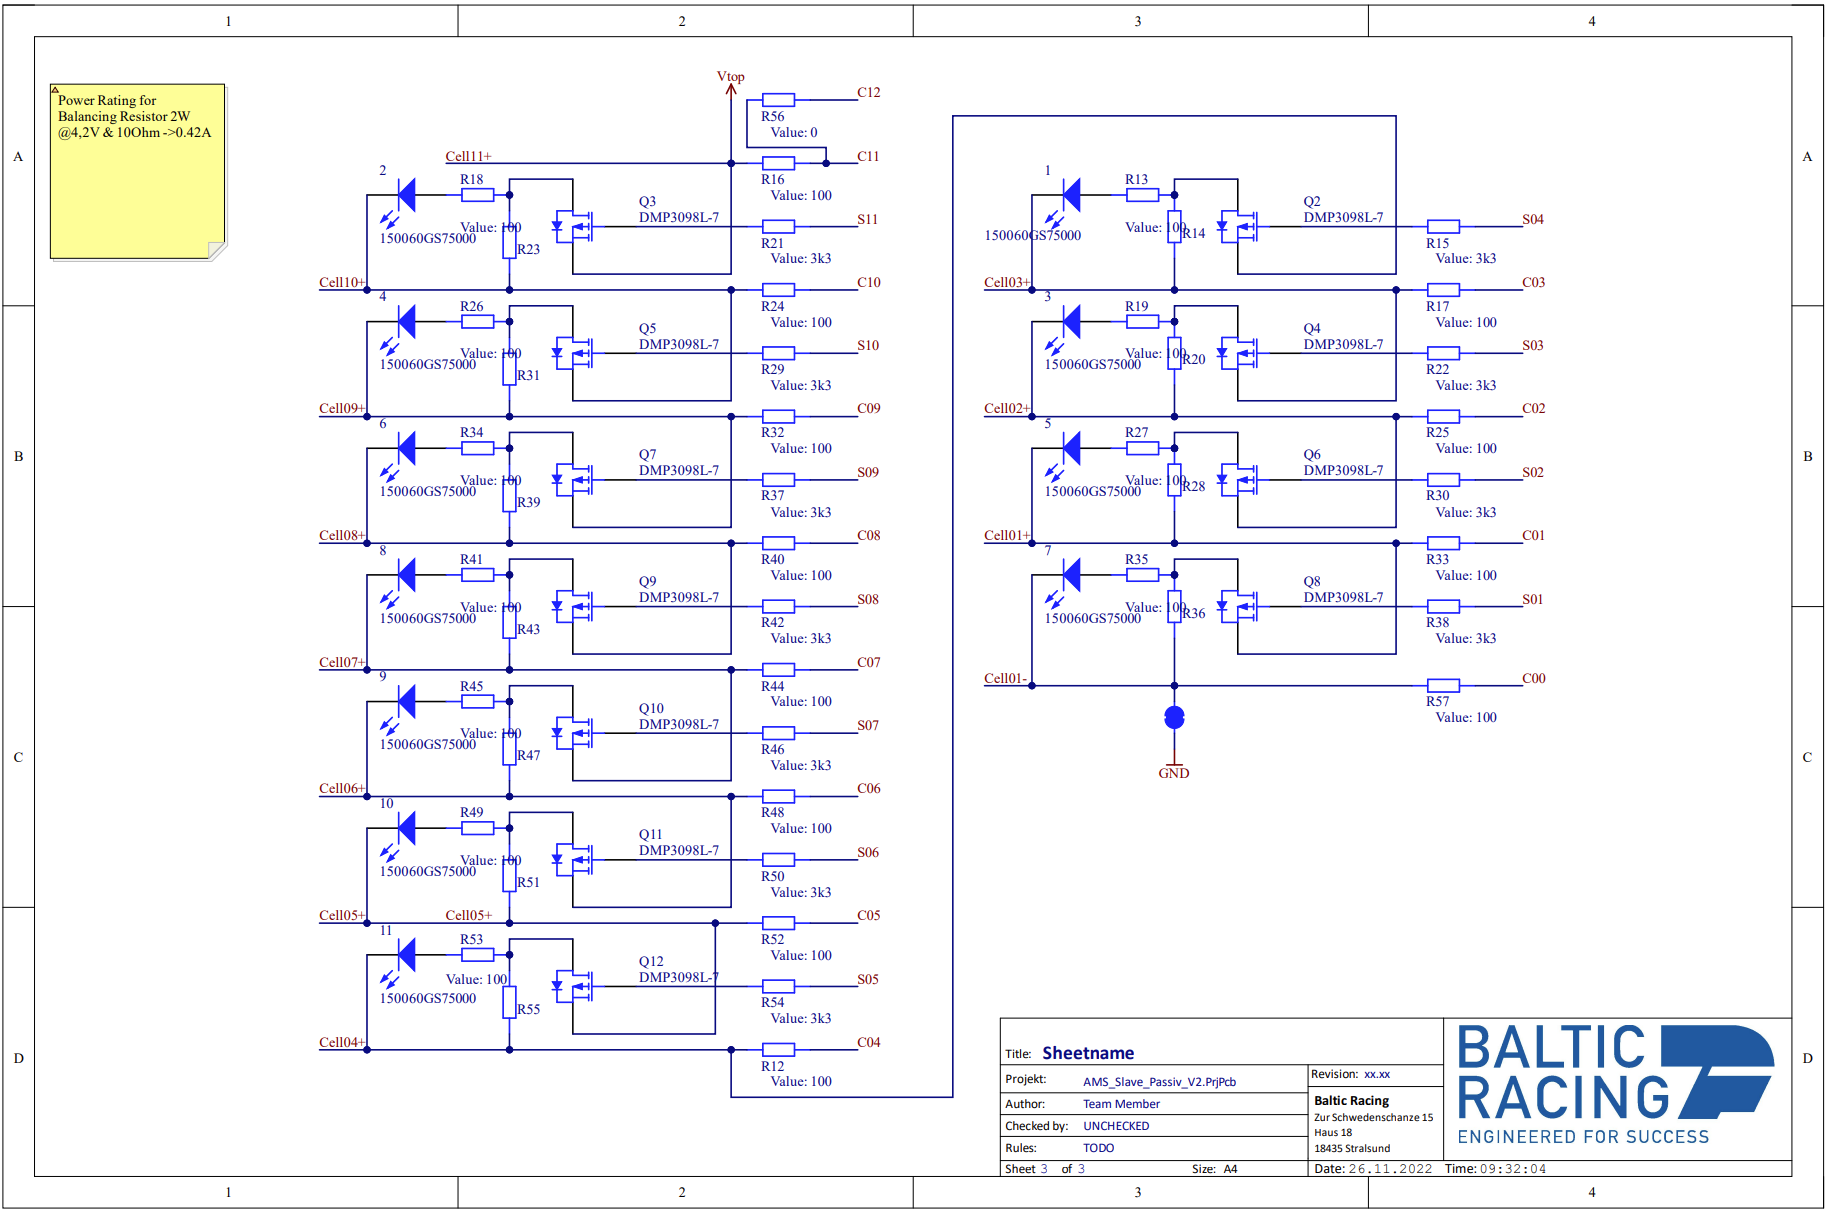
\includegraphics[width=0.7\linewidth]{bilder/AMS_Balancing_Schematic}
	\caption{Schaltplan \ac{AMS} Balancing}
	\label{fig:amsbalancingschematic}
\end{figure}

\FloatBarrier
\subsubsection{\ac{HV}-Indicator}

\begin{figure}
	\centering
	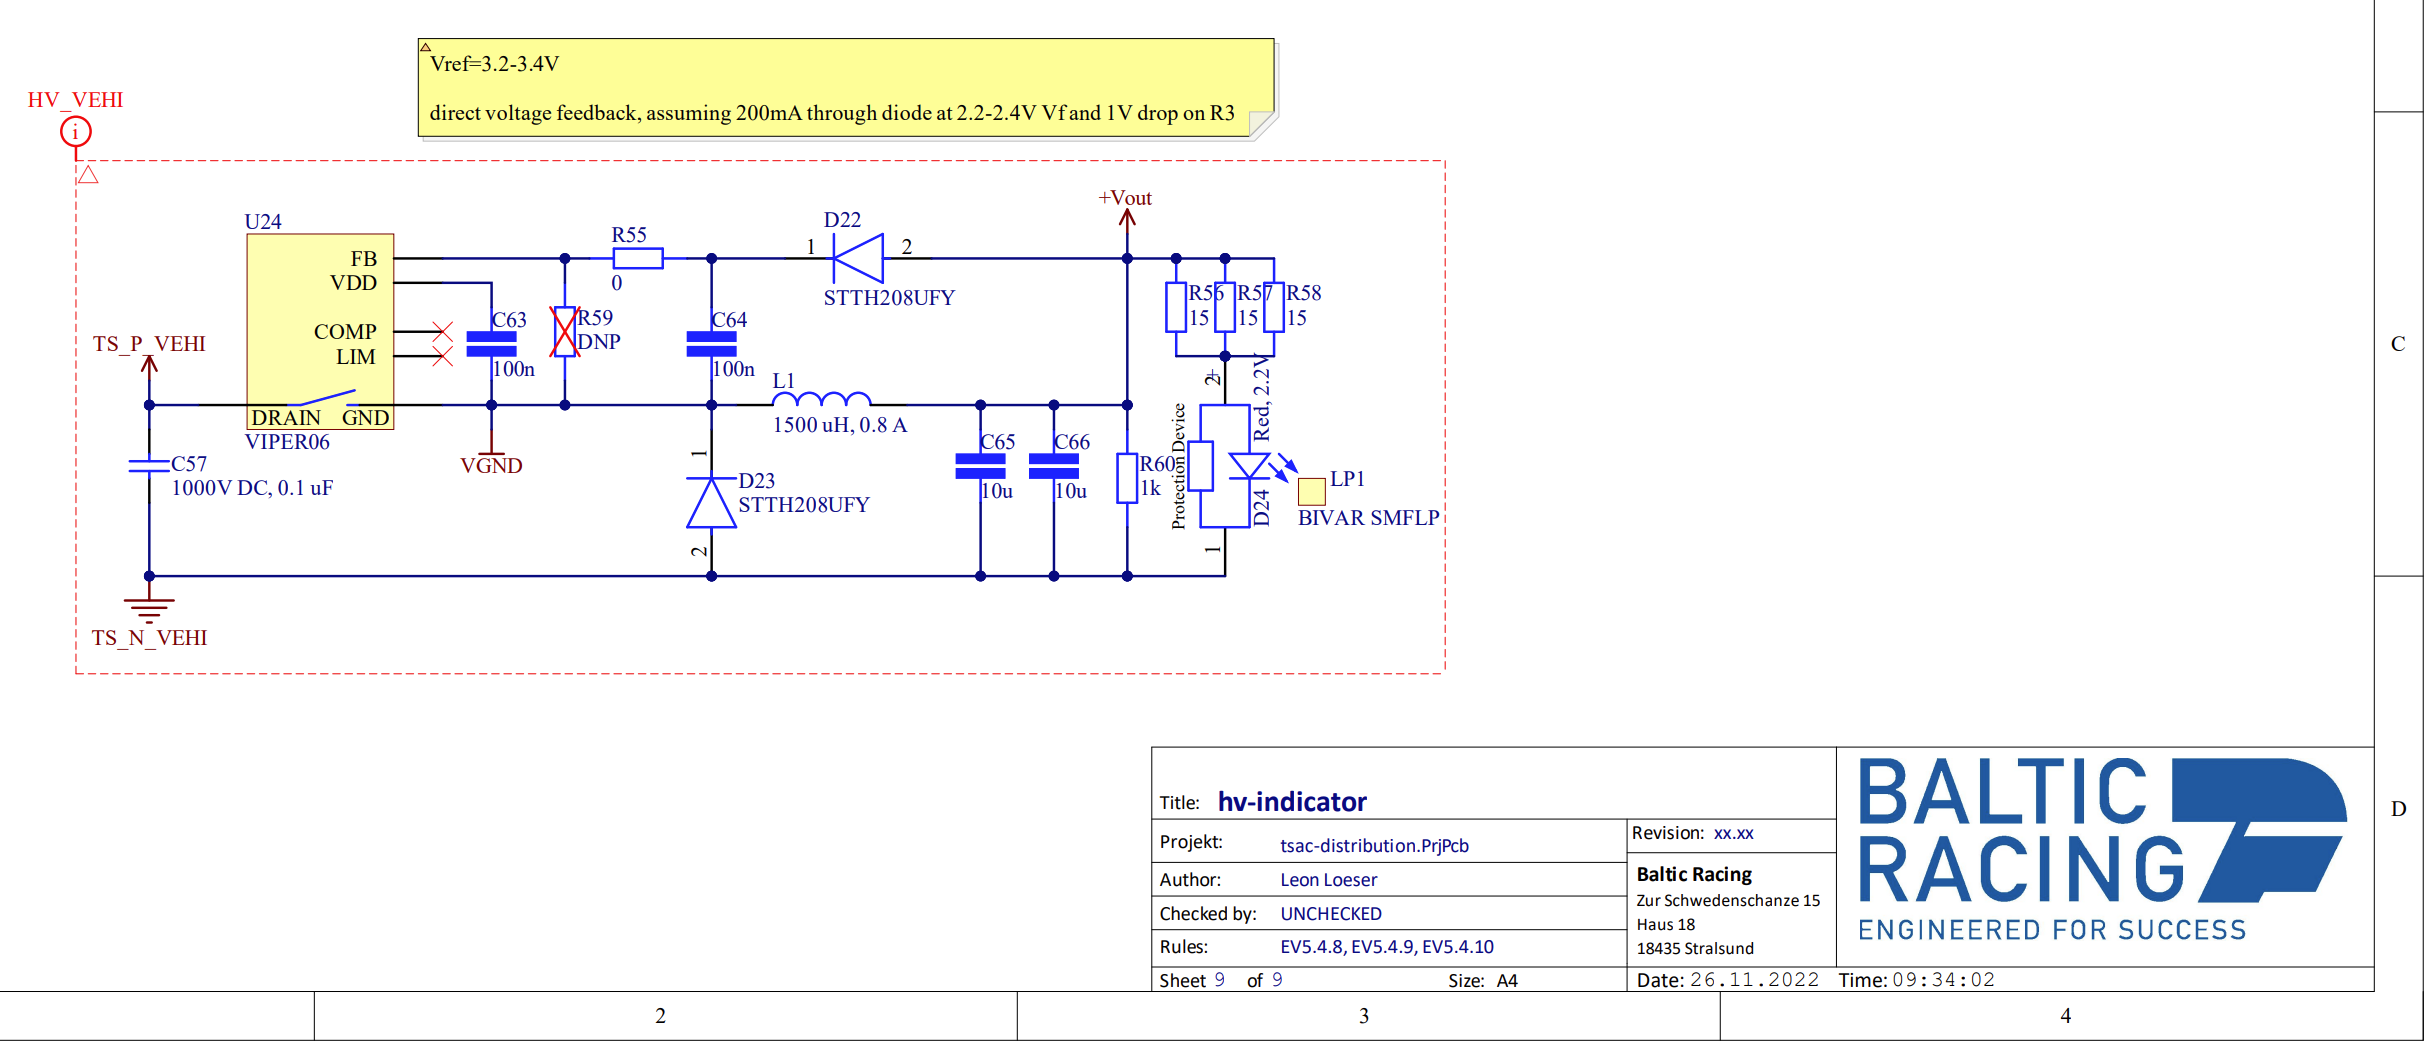
\includegraphics[width=0.7\linewidth]{bilder/HV_indicator_schematic}
	\caption{Schaltplan \ac{HV}-Indicator}
	\label{fig:hvindicatorschematic}
\end{figure}

Der \acfirst{HV} Indikator ist ein rotes Licht auf dem Akkumulator. Sofern an den \ac{HV}-Terminals des Akkus eine gefährliche Spannung liegt muss dieses Licht erleuchten und dem Bediener somit anzeigen das es z.b. nicht sicher ist den Akku vom Zwischenkreis zu trennen, da dieser noch unter Spannung steht. Die Anzeige erfolgt über eine Rote \ac{LED} wessen Licht mit einer Glasfaser von der Platine zum Deckel des Akkus geleitet wird. Die Ansteuerung der \ac{LED} erfolgt über einen kleinen \acfirst{DC}-Wandler, den Viper 06. Dieser Wandler verfügt über eine drain source startup voltage von \ensuremath{25-40V} \cite{Viper06}. Das bedeutet, bei einer Spannung in diesem Bereich beginnt der Chip zu arbeiten. Dieser Strom fließt dann zur \ac{LED}, so das diese zu leuchten beginnt. Die Feedback Schaltung ist direkt an den Spannungsausgang gekoppelt so das wir die interne Spannungsreferenz von \ensuremath{3,2 V - 3,4 V} nutzen. Die Vorwiderstände vor der \ac{LED} sind dementsprechend ausgelegt.

\FloatBarrier
\subsubsection{\ac{HV}-Messung}
Sinn der \ac{HV} Messung ist es, die Spannung welche am Akku als auch am Zwischenkreis anliegt, erfassen und digitalisieren zu können. Dadurch kann zusammen mit dem Signal vom Stromsensor z.b. die \ac{DC}-Leistung bestimmt und geloggt werden. 

\begin{figure}
	\centering
	\includegraphics[width=0.4\linewidth]{"bilder/Blockdiagramm ADUM3190"}
	\caption{Blockdiagramm ADUM 3190}
	\label{fig:blockdiagramm-adum3190}
\end{figure}

\begin{figure}
	\centering
	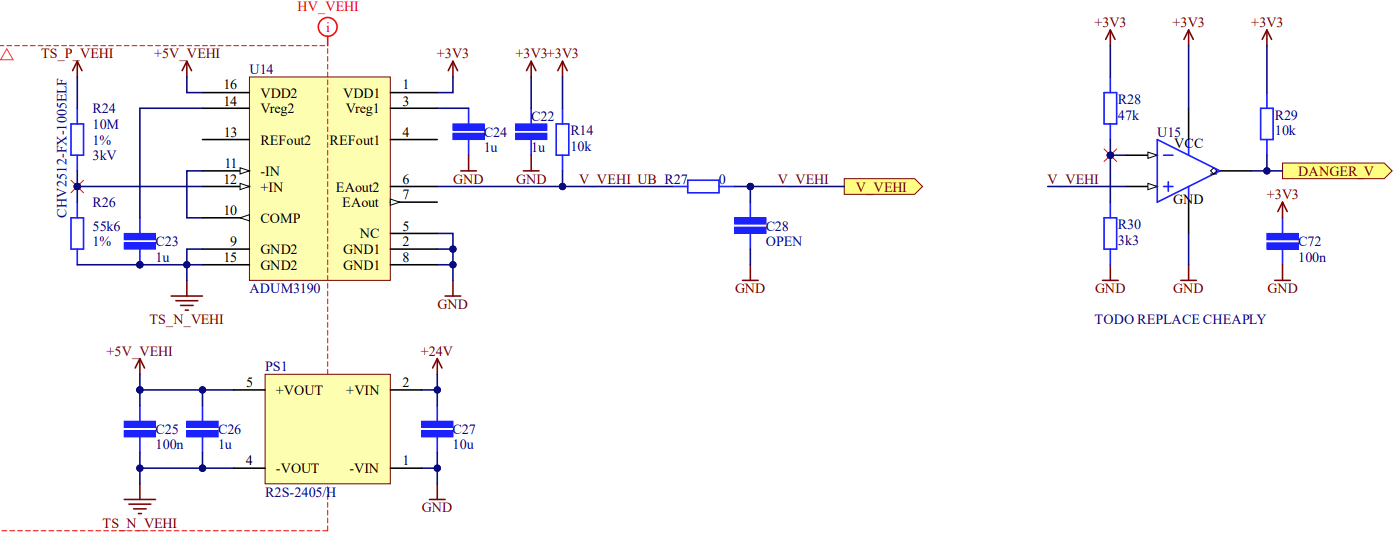
\includegraphics[width=0.9\linewidth]{bilder/HV_Measurement_PNG}
	\caption{Schaltplan \ac{HV}-Messung}
	\label{fig:hvmeasurementpng}
\end{figure}

Kern dieser Schaltung ist der ADUM 3190. Dabei handelt es sich um einen \ac{Iso}-\acfirst{OPV}. Der positive Eingang ist über einen Spannungsteiler mit dem \ac{HV}-Kreis verbunden. Der negative Eingang ist mit dem Ausgang des \ac{OPV} rückgekoppelt so das ein Spannungsfolger mit einer Verstärkung von 1 entsteht. Aus dem \ensuremath{10 M\Omega} und dem \ensuremath{55,6 k\Omega} Widerstand ergibt sich ein Verhältnis von \ensuremath{179,86 V} im \ac{HV}-Kreis zu einem Volt am Eingang des \ac{OPV}. Das ergibt eine maximale Eingangsspannung für die Schaltung von \ensuremath{593,54 V} da hierbei eine Ausgangsspannung von \ensuremath{3,3 V} erreicht wird. Bei dem R2S-2405/H handelt es sich um einen isolierten \ac{DC}-Wandler um den Chip \ac{HV}-seitig mit Strom zu versorgen. Die Komparatorschaltung um U15 gibt bei überschreiten der gefährlichen Spannung einen High-Pegel aus. Die Spannung über den positiven Eingang der Komparatorschaltung liegt bei \ensuremath{0,232 V} so das bei einer \acfirst{TS}-Spannung von größer \ensuremath{41,73 V} der High-Pegel anliegen sollte. Laut Regelwerk sollte dieser Pegel bei kleiner \ensuremath{60V} anliegen.

\FloatBarrier
\subsubsection{\ac{IMD} Monitoring}

Bei dem \acfirst{IMD} handelt es sich um ein Bender Isometer IR155-320x \cite{ISOMETERIR155-3203/IR155-3204}. Dieses Isolationsmessgerät wird von der Formula Student empfohlen und wird den Teams \ac{idR} von dem Unternehmen kostenlos zur Verfügung gestellt.
Das \ac{IMD} hat zwei Ausgänge die für die Auswertung des Messergebnisses relevant sind. Einmal ein digitales OK-HS-Signal und ein \acfirst{PWM}-Signal M\textsubscript{hs} oder M\textsubscript{ls} je nach Variante. Das OK-Signal gibt alle relevanten Informationen in der Form aus das es low geht wenn z.b ein Isolationsfehler oder ein Gerätefehler erkannt wurde. Das \ac{PWM}-Signal ermöglicht es den Fehler weiter einzugrenzen oder den aktuellen Messwert auszugeben. Dementsprechend muss das OK-Signal rein analog den \acfirst{SDC} betätigen können während der \ac{PWM}-Ausgang nur als Informationsquelle dient und an einen Mikrocontroller angeschlossen werden darf.
\\
\\
Beim Startup ist das PRE- als auch das CLR-/Signal am D-FlipFlop U7\textsubscript{A} low. Dadurch ist der Ausgang Q high was aufgrund der Diode D14 aber keinen Einfluss auf die restliche Schaltung hat. Die Spannung am Gate des P-Channel-Mosfet Q3 ist low und die Spannung an der Source ist high, dadurch liegt eine negative Gate-Source Spannung an so das der Mosfet geschlossen ist. Dementsprechend ist die Spannung an der Source annähernd low. Nun sollte, sofern kein Fehler seitens des \ac{IMD} vorliegt das OK-Signal high gehen. Dadurch öffnet der Fet Q3, gleichzeitig bleibt Q vom FlipFlop high. Nun liegt Spannung an der Basis von Q5 und es fließt ein Basis-Emitter-Strom so das auch ein Kollektor-Emittor-Strom fließen kann. Dadurch liegt zusammen mit den Widerständen R37 und R38 eine negative Gate-Source-Spannung an Q4 an, so das der P-Channel-Mosfet durchschaltet und der \ac{SDC} geschlossen wird. Daraufhin schaltet der \acfirst{POR} high so das der Zustand vom FlipFlop gespeichert wird und somit high bleibt. Wenn das Ok-Signal nun low geht weil ein Fehler auftritt, wird Q auf low gesetzt. Wenn OK nun wieder high geht weil z.b. der Fehler wieder aufgehoben ist, beispielsweise durch einen Wackelkontakt an einem der Messeingänge, wird der aktuelle Zustand gespeichert welcher low ist, so das die Schaltung sich nicht mehr selbst zurücksetzen kann. Ein Wiedereinschalten ist nur durch einen Power Cycle möglich.

\begin{figure}
	\centering
	\includegraphics[width=0.9\linewidth]{"bilder/IMD Monitoring schematic"}
	\caption{Schaltplan IMD Monitoring}
	\label{fig:imd-monitoring-schematic}
\end{figure}

\FloatBarrier
\subsection{\ac{HV}-\ac{DC}-\ac{DC}}
Bei der Topologie des \ac{HV}-\ac{DC}-\ac{DC}-Wandlers handelt es sich um einen active clamp forward transformer oder auch einen Eintaktflusswandler mit Entmagnetisierung des Trafokerns über eine Fangschaltung aus Mosfet, Widerstand und Kondensator. Man hat sich speziell für diese Fangschaltung und nicht für einen Transformator mit Entmagnetisierungsspule entschieden da man so aus dem Bereich des Sonderangefertigten-Transformators rauskommt. Bisher wurden im Rahmen des Formula Student Projektes nur \ac{DC}-Wandler ohne galvanische Trennung eingesetzt. Dabei handelte es sich in der Regel um den klassischen Auf- oder Abwärts-/Wandler. Die Topologie des Eintaktflusswandler ist bei diesem Leistungsbereich nach Aussage einiger Hersteller für die relevanten \ac{IC}`s zwar an der obersten Grenze dessen was sinnvoll möglich ist, zeichnet sich aber durch seine große Ähnlichkeit zum nicht galvanisch getrennten Abwärtswandler und damit seine verhältnismäßige Einfachheit aus. Folgend der vereinfachte Aufbau beider Wandlertopologien in den Abbildungen \ref{fig:buckconverter} und \ref{fig:forwardconverter} zur Gegenüberstellung.

\begin{figure}
	\centering
	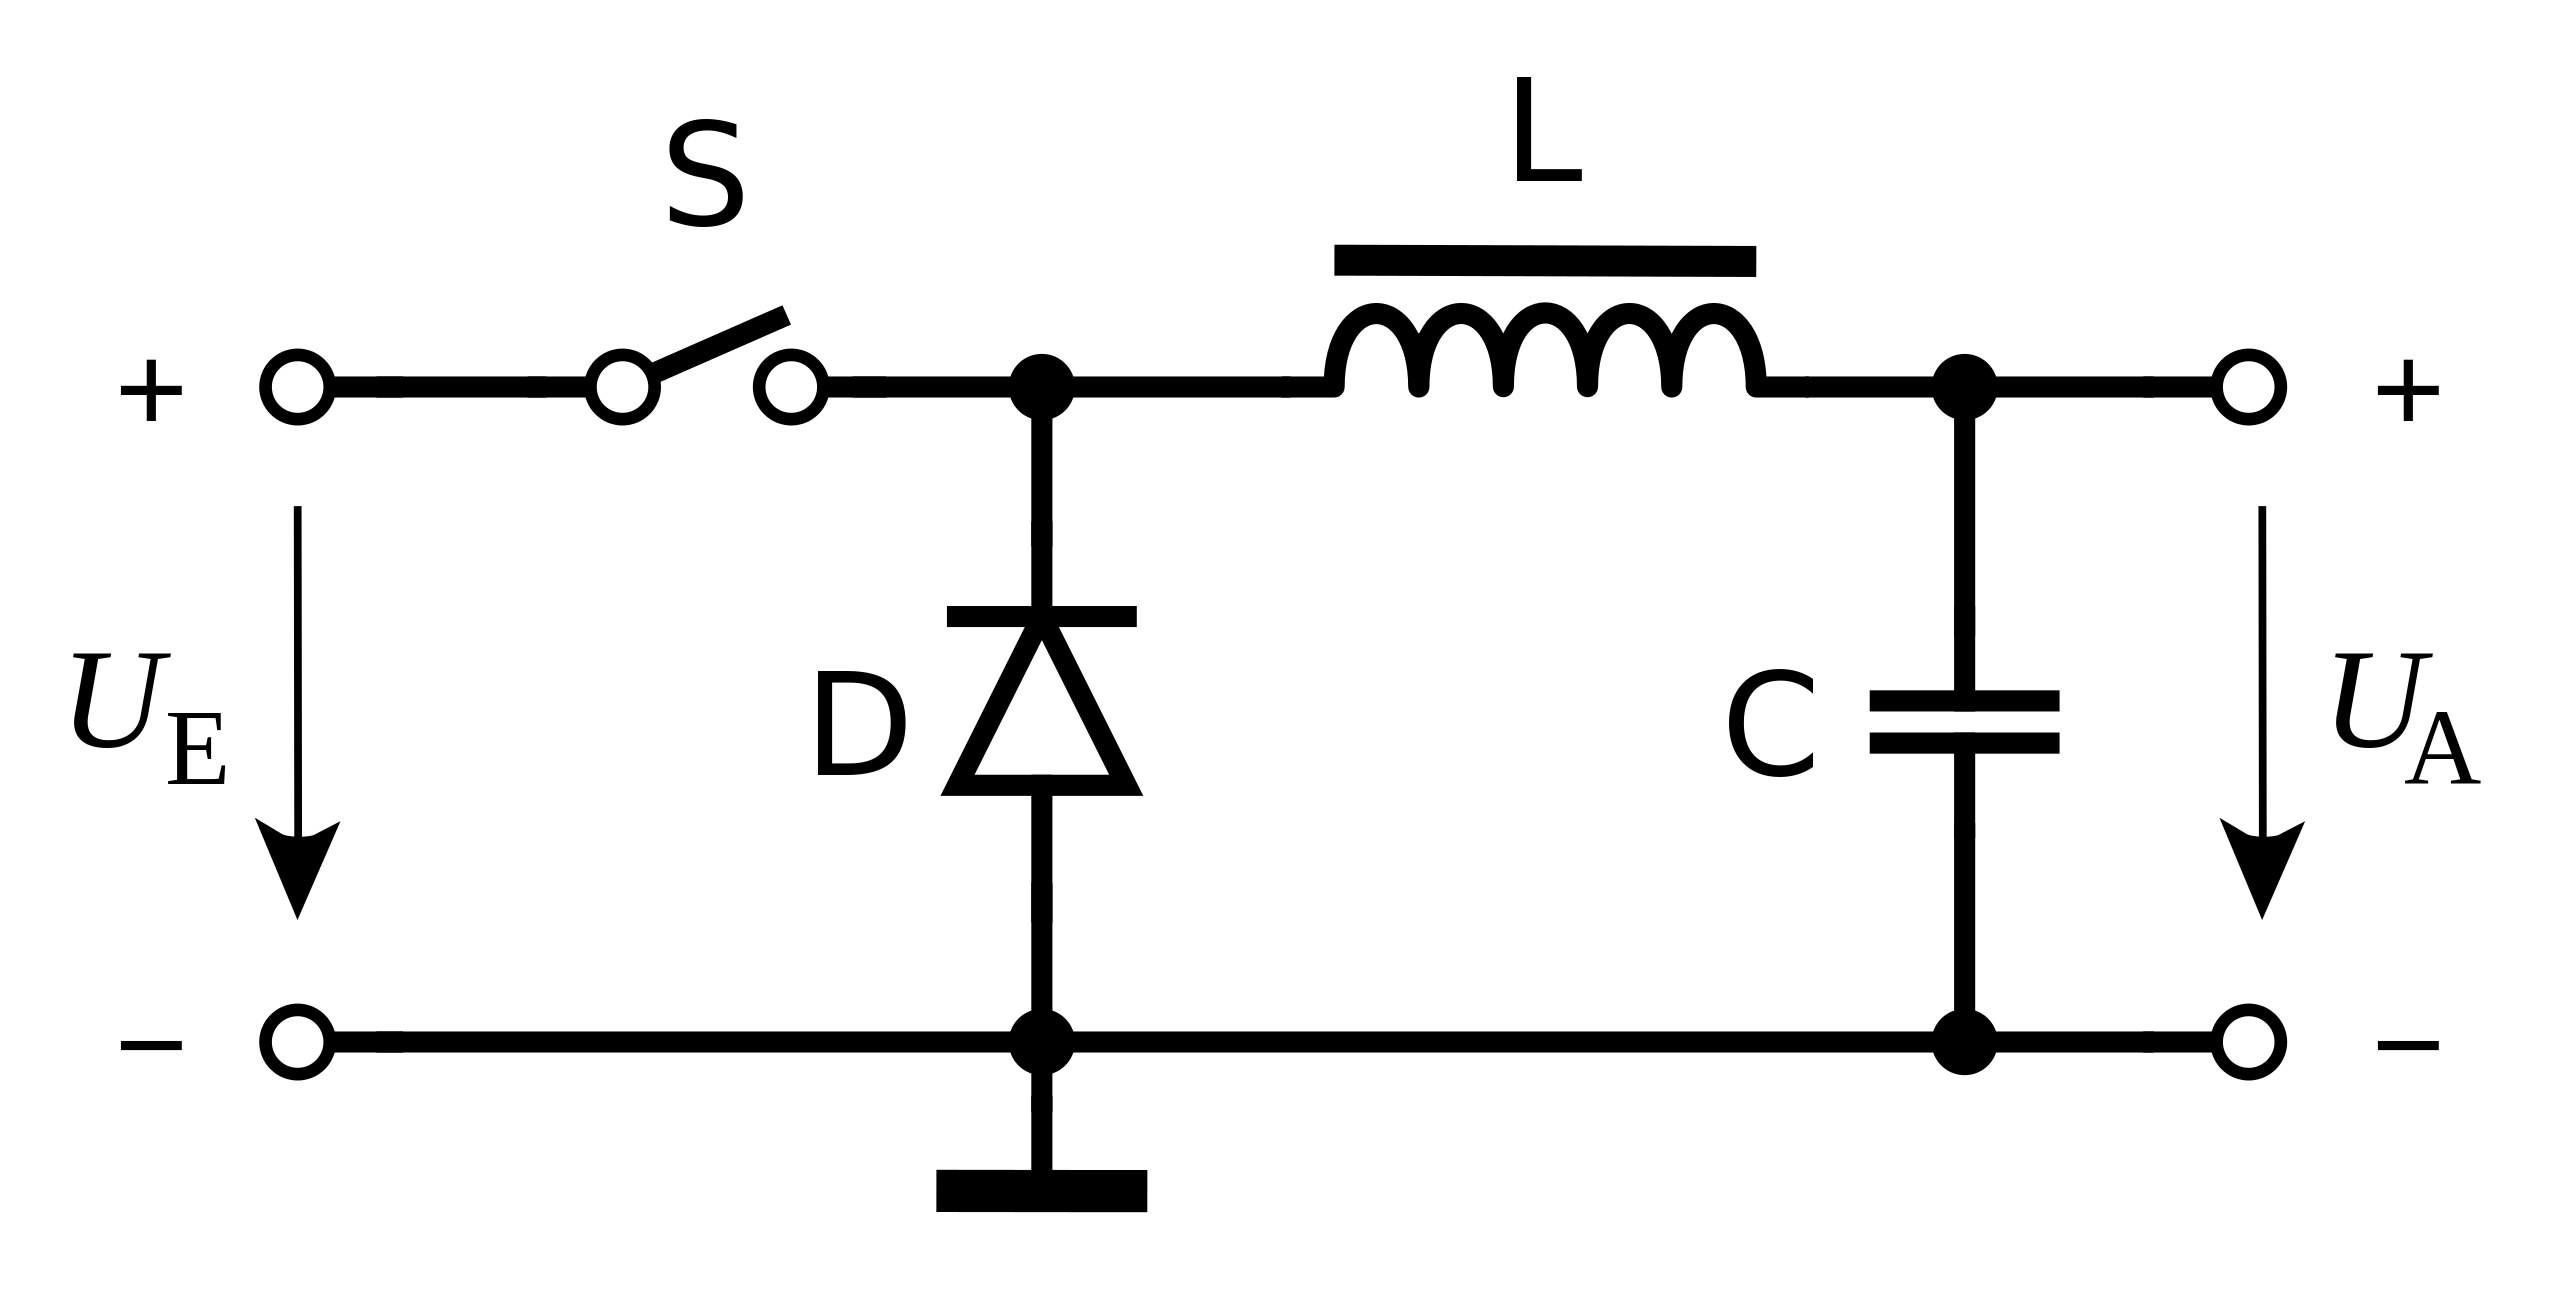
\includegraphics[width=0.5\linewidth]{bilder/Buck_converter.svg}
	\caption{Buck Konverter Topologie \cite{WikiWandlertopo}}
	\label{fig:buckconverter}
\end{figure}

\begin{figure}
	\centering
	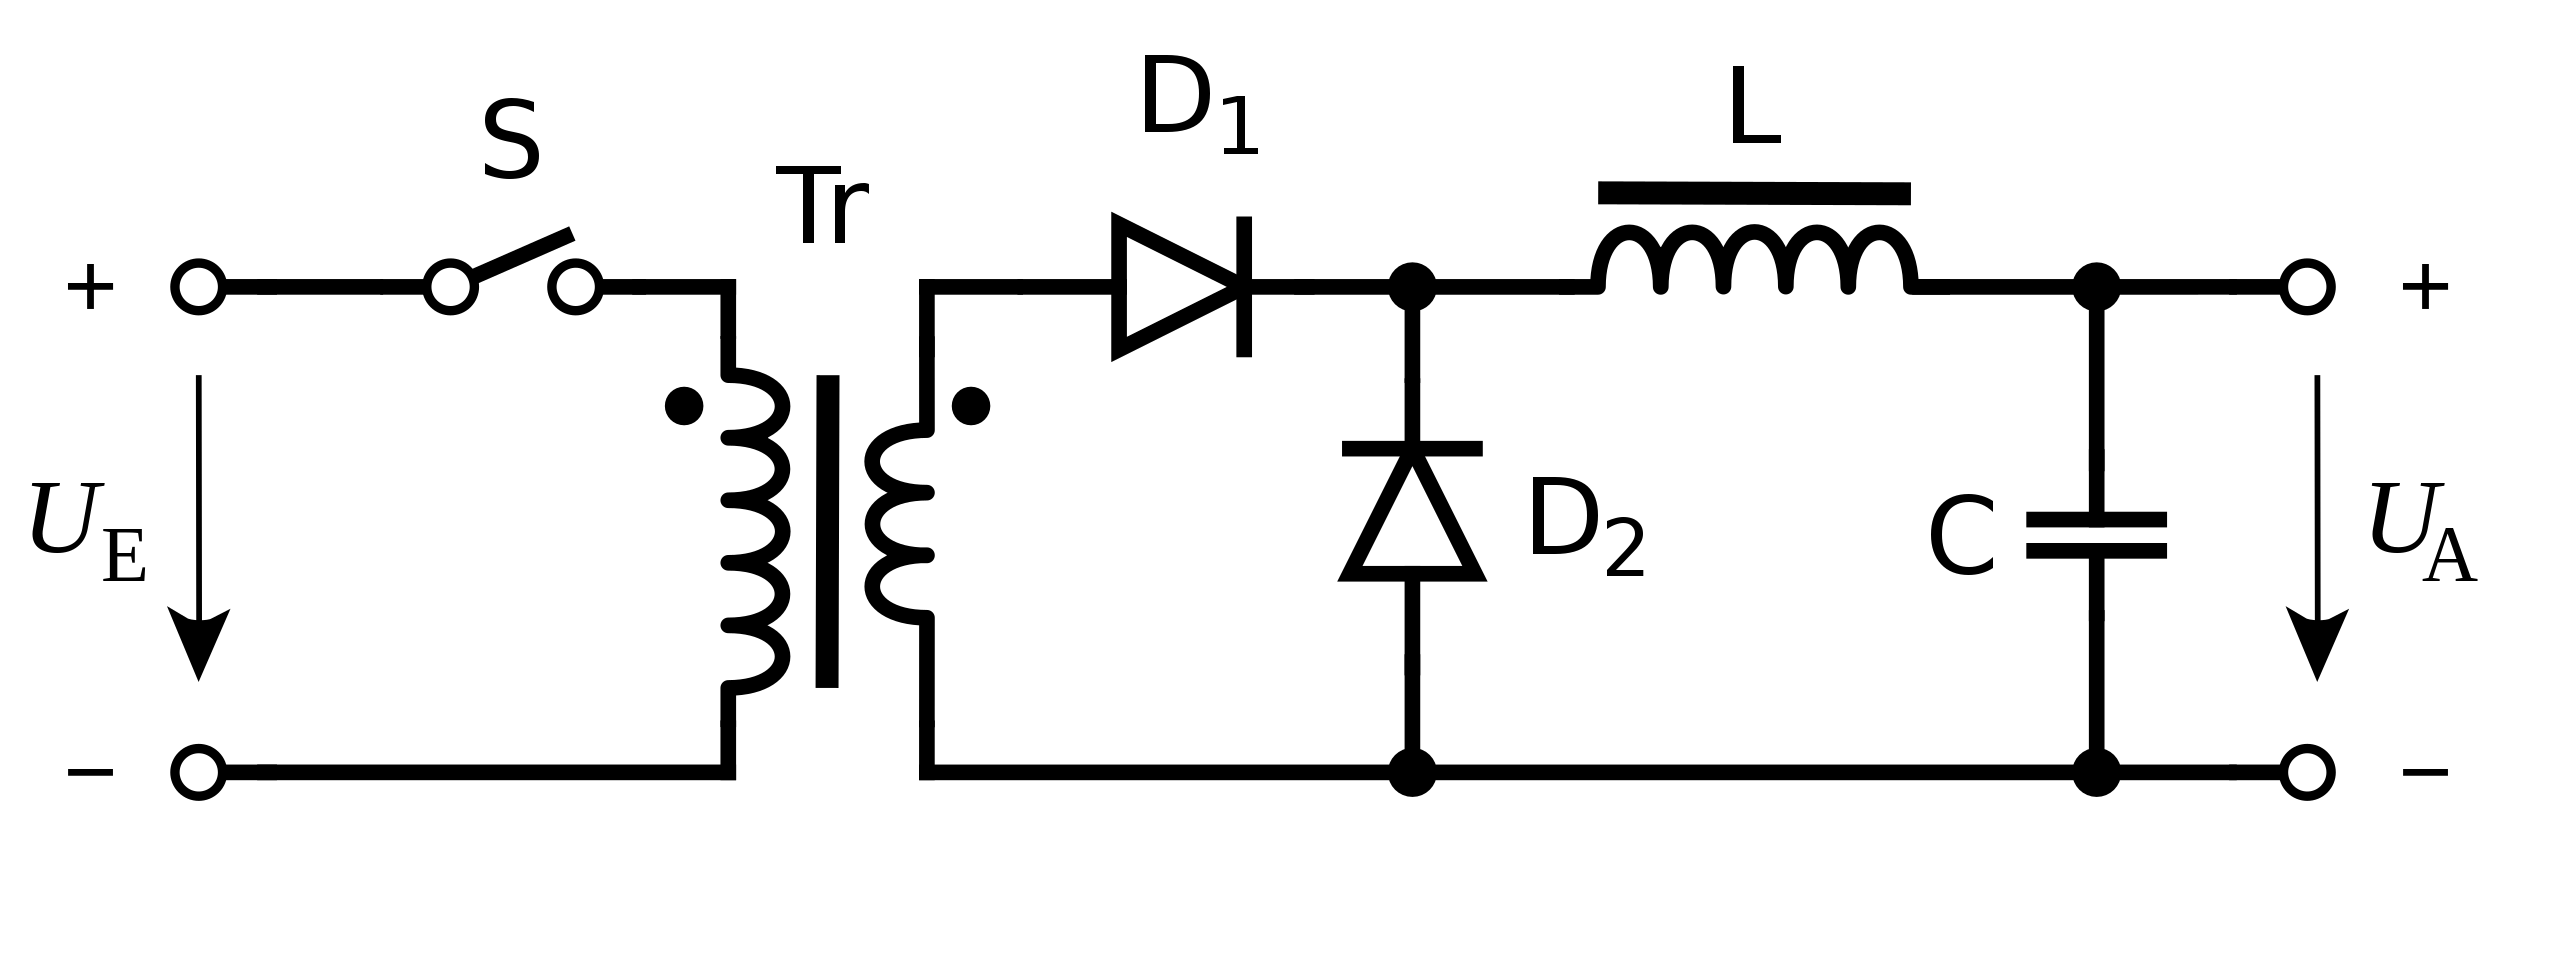
\includegraphics[width=0.5\linewidth]{bilder/Forward_converter.svg}
	\caption{Eintaktflusswandler Topologie \cite{WikiWandlertopo}}
	\label{fig:forwardconverter}
\end{figure}

Von der Firma Linear Technology existiert ein \ac{IC}, der LT 3752 \cite{LT3752LT3752-1}. Dieser ist speziell für den Aufbau von Wandlern dieser Topologie gedacht. Weiter existiert die Demo Schaltung DC 1929A \cite{DC1929A} basierend auf diesem \ac{IC}. Hierbei handelt es sich um einen \ensuremath{400 V} zu \ensuremath{12 V} Wandler mit einer Ausgangsleistung von \ensuremath{200 W}. Das hier vorliegende Design wurde mithilfe des Datenblattes, des LT 3752, des LT 8311 \cite{LT8311} und mithilfe der Schaltpläne als auch der Layout Dateien des DC 1929A erstellt.
\\
\\
Zur Auflistung der Ausgangsparameter.

\begin{table}
	\centering
	\caption{Ausgangsparameter \ac{DC}\ac{DC} Wandler}
	\begin{tabular}{|c|c|c|c|}
		\hline
		Parameter & Wert & Einheit &Kommentar \\
		\hline
		\glsc{symb:V_out} & 24 & V & Boardnetzspannung \\
		\hline
		\glsc{symb:P_out} & 960 & W & Leistungsverbrauch LV System Maßgeblich Lüfter\\
		\hline
		\glsc{symb:V_inmin} & 230 & V & 2 V Entladeschluss plus Sicherheit \\
		\hline
		\glsc{symb:V_inmax} & 630 & V & 4,25 V Ladeschluss plus Sicherheit \\
		\hline
		\glsc{symb:I_out} & 40 & A &\\
		\hline
		\glsc{symb:f_osc} & 100 & kHz & Basiert auf Referenzdesign\\
		\hline
		Foldback Ratio & 2 & - & Datenblatt\\
		\hline
		\glsc{symb:INTV_CC} & 10 & V & \\
		\hline
		\glsc{symb:t_amb} & 50 & \ensuremath{^\circ C} & angenommen\\
		\hline
		\glsc{symb:t_max} & 125 & \ensuremath{^\circ C} & max. Temperatur für Automotive Komponenten\\
		\hline
	\end{tabular}
\end{table}

Mit diesen Werten muss nun ein passender Transformator gefunden werden. Hierfür wurden diverse Hersteller kontaktiert. Bei der Firma Champs Technologies gab es eine erfolgreiche Rückmeldung in der Form, dass Sie einen Transformator im Angebot habend der für unsere Anwendung relativ gut passt, den R41-AC-2202.
\\
\\
Zur Kontrolle können wir eine Rechnung durchführen. Der maximale Duty Cycle \glsc{symb:D_max} liegt laut Datenblatt typischerweise bei \ensuremath{60\%}.
\\
\\
Hiermit könne wir nun das ideale Wicklungsverhältnis bestimmen

\begin{equation}
	\glsc{symb:NP/NS_ideal} = \dfrac{\glsc{symb:V_inmin}}{\glsc{symb:V_out}}*\glsc{symb:D_max_ideal}
\end{equation}

Dann brauchen wir zum Vergleich das reale Verhältnis von Primär- zu Sekundär-/Wicklungen.

\begin{equation}
	\glsc{symb:NP/NS} = \dfrac{1}{\glsc{symb:NS/NP}}
\end{equation}

Indem wir nun 2 Transformatoren mit der Primärseite in Parallel und der Sekundärseite in Reihe verschalten können wir das Wicklungsverhältnis halbieren.

\begin{table}[h]
	\centering
	\caption{Berechnung Wicklungsverhältnis}
	\begin{tabular}{|c|c|c|}
		\hline
		\multicolumn{3}{|c|}{Eingangsparameter}\\
		\hline
		\glsc{symb:NS/NP} & 0,091 & \ensuremath{-} \\
		\hline
		\multicolumn{3}{|c|}{Ergebnisse} \\
		\hline
		\glsc{symb:NP/NS_ideal} & 5,75 & \ensuremath{-}   \\
		\hline
		\glsc{symb:NP/NS} & 5,495 & \ensuremath{-}   \\
		\hline
	\end{tabular}
\end{table}

Nun können wir den minimalen und maximalen Duty Cycle bestimmen. Dieser lässt sich für den Betrieb über folgende Gleichung ermitteln.

\begin{equation}
	\label{minimaler duty cycle}
	\glsc{symb:D_min} = \dfrac{\glsc{symb:V_out}}{\glsc{symb:V_inmax}}*\glsc{symb:NP/NS} = 20,93\%
\end{equation}

\begin{equation}
	\label{maximaler duty cycle}
	\glsc{symb:D_max} = \dfrac{\glsc{symb:V_out}}{\glsc{symb:V_inmin}}*\glsc{symb:NP/NS} = 57\%
\end{equation}

Im folgenden soll nun die Auslegung von Ausgangs Induktivität (L1 \& L2) als auch Kapazität (C13 - 15) erfolgen. Hierfür benötigen wir zu Berechnung der Induktivität den Ripple-Strom an der Induktivität. Als Faustregel kann man diesen mit \ensuremath{20-40 \%} vom maximalen Strom annehmen. Ziel der Induktivität ist es aus den einzelnen Stromimpulsen der Schaltstufe einen konstanten Ausgangsstrom zu erzeugen. Je größer diese Impulse sind, desto größer muss die entsprechende Induktivität gewählt werden. Wir wollen das der Wandler die meiste Zeit im \acfirst{CCM} arbeitet, heißt der Wandler arbeitet mit fester Arbeitsfrequenz und variiert den Duty Cycle. Der \acfirst{DCM} wird erreicht wenn der Stromverbrauch des Systems kleiner ist als der Ripple-Strom in der Induktivität. Hierbei werden einzelne Pulse ausgelassen und somit die Schaltfrequenz reduziert. Dies führt allerdings wie man an den Formeln im folgenden feststellen kann dazu das der Ausgangsripple steigt bzw. je nach Lastzustand variiert. Eine Abhilfe schafft hier der \acfirst{FCCM}, hier wird auch im Bereich wo der Wandler normalerweise im \ac{DCM} arbeiten würde trotzdem im \ac{CCM} gearbeitet. Dabei erlauben wir aber einen Negativen Strom in der Ausgangsinduktivität und somit höhere Verluste und Anforderung an die Sekundärseitigen Fet`s. Aber wir ermöglichen eine konstant hohe Arbeitsfrequenz und damit einen stabileren Ausgang. Daher fiel hier die Entscheidung auf den \ac{FCCM}. Der minimale Stromverbauch für das Fahrzeug wurde ermittelt indem alle Datenblatt Stromverbräuche der einzelnen Systeme aufaddiert wurden und liegt bei ca. \ensuremath{4 A} respektive \ensuremath{100 W}.

\begin{equation}
	\glsc{symb:L_O} = (1-((1/\glsc{symb:V_inmax})*\glsc{symb:NP/NS}*\glsc{symb:V_out}))*\dfrac{1}{\glsc{symb:I_Ripple}}*\glsc{symb:V_out}*\dfrac{1}{\glsc{symb:f_osc}}
\end{equation}

Das Ergebnis der Berechnung der Ausgangsinduktivität sind \ensuremath{47,44 uH}. Für diese Induktivität könnte man vier AGP4233-153ME der Firma Coilcraft zusammenschalten um auf \ensuremath{60 uH} zu kommen. Diese sind jedoch viel zu groß für den Bauraum so das die größtmögliche in den Bauraum passende Spulenkombination gewählt wurde. Hierbei handelt es sich um vier AGM2222-562ME die zusammen \ensuremath{22,4uH} mitbringen. Hiermit könne wir nun den neuen Ripple-Strom bestimmen welchen wir für die Auslegung des Kondensators brauchen.

\begin{equation}
	\glsc{symb:I_Ripple} = \dfrac{\glsc{symb:V_out}}{\glsc{symb:L_O}*\glsc{symb:f_osc}} * 1 - \dfrac{\glsc{symb:V_out}} {\glsc{symb:V_inmax}} * \glsc{symb:NP/NS}
\end{equation}

Die Ripple-Spannung \glsc{symb:V_Ripple} wird auf \ensuremath{1\%} der Ausgangsspannung festgelegt \ensuremath{(0,24 V)}. Nun brauchen wir noch den \acfirst{ESR} der Kondensatoren welche verwendet werden sollen. Es ist gängige Praxis einige Keramik Kondensatoren mit niedrigem \ac{ESR} zu verwenden und ein größeren \acfirst{Elko} zur Dämpfung größere Last-transienten. Diese Rechnung würde man nun mit einem angenommenen typischen \ac{ESR} von z.b \ensuremath{3 m\Omega} durchführen und Sie dann für die tatsächlichen Werte wiederholen, wenn entsprechende Kondensatoren ausgewählt wurden. Bei vielen Kondensatoren ist im Datenblatt oft nur ein \acfirst{DF} angegeben, in diesem Fall sollte man beim Hersteller nach weiteren Informationen suchen. So hat die Firma \acfirst{WE} Diagramme zur \ac{ESR} in ihrem separatem Tool, dem Red Expert. In der Abbildung \ref{fig:we-esr-cap} ein Beispiel wie solch ein Diagramm aussehen kann.

\begin{figure}
	\centering
	\includegraphics[width=0.4\linewidth]{"bilder/WE ESR Cap"}
	\caption{\ac{ESR} Kondensator}
	\label{fig:we-esr-cap}
\end{figure}

\begin{equation}
	\glsc{symb:C_O} = \dfrac{\glsc{symb:I_Ripple}}{(8*\glsc{symb:f_osc}*(\glsc{symb:V_Ripple}-\glsc{symb:I_Ripple}*\glsc{symb:ESR}))}
\end{equation}

\begin{table}[h]
	\centering
	\caption{Berechnung Ausgangs- Kapazität und Induktivität}
	\begin{tabular}{|c|c|c|}
		\hline
		\multicolumn{3}{|c|}{Eingangsparameter}\\
		\hline
		\glsc{symb:I_Ripple} & 4 -> 8,47 & \ensuremath{A}  \\
		\hline
		\glsc{symb:V_Ripple} & 0,24 & \ensuremath{V} \\
		\hline
		\glsc{symb:ESR} & 1,6 & \ensuremath{m\Omega} \\
		\hline		
		\multicolumn{3}{|c|}{Ergebnisse} \\
		\hline
		\glsc{symb:L_O}1 & 47,44 -> 22,4 & \ensuremath{uH} \\
		\hline
		\glsc{symb:C_O}1 & 45,334 & \ensuremath{uF} \\
		\hline
	\end{tabular}
\end{table}

Für die Kapazität werden zwei \ensuremath{22 uF} \acfirst{MLCC}`s und ein \ensuremath{2,2 mF} \ac{Elko} der Firma \ac{WE} in parallel verschaltet.\\
\\
Nun folgt die Berechnung der Fangschaltung bestehend aus Clamp Kondensator und einem RC Snubber (C16 - C18 \& C20 - C22 \& R15).

\begin{equation}
	\glsc{symb:C_CL} = \dfrac{10}{\glsc{symb:H_Prim}} * (\dfrac{1-\glsc{symb:D_min}}{2*\pi*\glsc{symb:f_osc}})^2
\end{equation}

mit \glsc{symb:H_Prim} in uH
\\
und \glsc{symb:f_osc} in kHz
\\
Nun können wir den Snubber mit folgenden Formeln aus dem Datenblatt berechnen.

\begin{equation}
	\glsc{symb:C_S} = 6 * \glsc{symb:C_CL}
\end{equation}

\begin{equation}
	\glsc{symb:R_S} = (\dfrac{1} {1 - \glsc{symb:D_max}} ) * \sqrt{\dfrac{\glsc{symb:H_Prim}} {\glsc{symb:C_CL}}}
\end{equation}
mit \glsc{symb:H_Prim} in H

\begin{table}[h]
	\centering
	\caption{Snubber Berechnung}
	\begin{tabular}{|c|c|c|}
		\hline
		\multicolumn{3}{|c|}{Eingangsparameter}\\
		\hline
		\glsc{symb:H_Prim} & 3900 & \ensuremath{uH}  \\
		\hline	
		\multicolumn{3}{|c|}{Ergebnisse} \\
		\hline
		\glsc{symb:C_CL}1 & 4,1 & \ensuremath{nF} \\
		\hline
		\glsc{symb:C_S}1 & 24,4 & \ensuremath{nF} \\
		\hline
		\glsc{symb:R_S}1 & 2297 & \ensuremath{\Omega} \\
		\hline
	\end{tabular}
\end{table}

Nun folgt die Berechnung der Schaltorgane, beginnend mit dem Primärseitigen Powerswitch (Q6) in Abbildung \ref{fig:hvdcdctransformerschematic}. Alle Formeln entstammen dem Datenblatt des LT 3752 \cite{LT3752LT3752-1}. Zu erst bestimmen wir die maximale Drain-Spannung wie folgt.

\begin{equation}
	\glsc{symb:V_DS} = \dfrac{\gls{symb:V_inmax}^2}{\gls{symb:V_inmax}-(\glsc{symb:V_out} * \glsc{symb:NP/NS})} * Sicherheit(20\%)
\end{equation}

Dann bestimmen wir die einzelnen Leistungsabfälle am Schalter.

\begin{equation}
	\glsc{symb:P_conduction} = \glsc{symb:NP/NS} * \dfrac{\glsc{symb:V_out}} {\glsc{symb:V_inmax}} * (\glsc{symb:NS/NP} * \glsc{symb:I_out})^2 * \glsc{symb:R_DS on}
\end{equation}

\begin{equation}
	\glsc{symb:P_Gatedriver} = \glsc{symb:Q_G} * \glsc{symb:INTV_CC} * \glsc{symb:f_osc}
\end{equation}

\begin{equation}
	\glsc{symb:P_Turn on} = \dfrac{1}{2} * \glsc{symb:I_out} * \glsc{symb:NS/NP} * \glsc{symb:V_DS} * \dfrac{\glsc{symb:Q_GD}}{\glsc{symb:I_Gate}} * \glsc{symb:f_osc}
\end{equation}

\begin{equation}
	\glsc{symb:P_Turn off} = \dfrac{1}{2} * \glsc{symb:I_out} * \glsc{symb:NS/NP} * \dfrac{\glsc{symb:V_inmax}}{1-\glsc{symb:D_max}} * \dfrac{\glsc{symb:Q_GD}}{\glsc{symb:I_Gate}} * \glsc{symb:f_osc}
\end{equation}

\begin{equation}
	\glsc{symb:P_gesamt} = \glsc{symb:P_conduction} + \glsc{symb:P_Gatedriver} + \glsc{symb:P_Turn off} + \glsc{symb:P_Turn off}
\end{equation}

Damit ergeben sich die Werte in Tabelle \ref{tab:Leistung am Primär Fet}

\begin{table}[h]
	\centering
	\caption{Leistung am Primär Fet}
	\label{tab:Leistung am Primär Fet}
	\begin{tabular}{|c|c|c|}
		\hline
		\multicolumn{3}{|c|}{Eingangsparameter}\\
		\hline
		\glsc{symb:R_DS on} & 0,225 & \ensuremath{\Omega}  \\
		\hline	
		\glsc{symb:Q_G} & 30 & \ensuremath{nC}\\
		\hline
		\glsc{symb:Q_GD} & 6 & \ensuremath{nC}\\
		\hline
		\glsc{symb:I_Gate} & 2 & \ensuremath{A}\\
		\hline
		\multicolumn{3}{|c|}{Zwischenergebnis} \\
		\hline			
		\glsc{symb:V_DS} & 959,13 & \ensuremath{V}\\
		\hline
		\glsc{symb:P_conduction}& 6,84 & \ensuremath{W}\\
		\hline
		\glsc{symb:P_Gatedriver}& 0,03 & \ensuremath{W}\\
		\hline
		\glsc{symb:P_Turn on}& 1,04 & \ensuremath{W}\\
		\hline
		\glsc{symb:P_Turn off}& 1,61 & \ensuremath{W}\\
		\hline
		\multicolumn{3}{|c|}{Ergebnisse} \\
		\hline
		\glsc{symb:P_gesamt} & 9,52 & \ensuremath{W} \\
		\hline
	\end{tabular}
\end{table}

Nun bestimmen wir die Temperatur am Fet indem wir die einzelnen thermischen Widerstände in Reihe schalten und mit der Leistung multiplizieren.

\begin{equation}
\glsc{symb:R_th_ges} = \glsc{symb:R_th_JC} + \glsc{symb:R_th_CS} + \glsc{symb:R_th_SA}
\end{equation}

\begin{equation}
	\glsc{symb:t_Fet} = \glsc{symb:P_gesamt} * \glsc{symb:R_th_ges} + \glsc{symb:t_amb}
\end{equation}

\glsc{symb:R_th_CS} ergibt sich aus der Kontaktfläche zwischen Fet und Kühlkörper sowie der Wärmedurchgangskoeffizient des Interface Materials. In diesem Fall wird die Wärmeleitpaste Arctic Silver 5 verwendet.

\begin{equation}
	\glsc{symb:R_th_CS} = \dfrac{1}{\glsc{symb:A_Sink} * \glsc{symb:U_th}} 
\end{equation}

Eingesetzt ergeben sich nun die Werte in der Tabelle \ref{tab:Temperatur am Primär Fet}

\begin{table}[h]
	\centering
	\caption{Temperatur am Primär Fet}
	\label{tab:Temperatur am Primär Fet}
	\begin{tabular}{|c|c|c|}
		\hline
		\multicolumn{3}{|c|}{Eingangsparameter}\\
		\hline
		\glsc{symb:R_th_JC} & 0,9 \cite{UJ3C120150K3S} & \ensuremath{K/W} \\
		\hline	
		\glsc{symb:R_th_CS} & 0,0089  & \ensuremath{K/W}\\
		\hline
		\glsc{symb:R_th_SA} & 3,9 \cite{RA-T2X-38E} & \ensuremath{K/W} \\
		\hline
		\glsc{symb:A_Sink} & 322,4 & \ensuremath{mm^2} \\
		\hline
		\glsc{symb:U_th} & 0,35 \cite{ArcticSilver} & \ensuremath{W/mm^2*K} \\
		\hline
		\multicolumn{3}{|c|}{Zwischenergebnis} \\
		\hline	
		\glsc{symb:R_th_CS} & 0,0089 & \ensuremath{K/W} \\		
		\hline
		\glsc{symb:R_th_ges} & 4,809 & \ensuremath{V} \\
		\hline
		\multicolumn{3}{|c|}{Ergebnisse} \\
		\hline
		\glsc{symb:t_Fet} & 95,80 & \ensuremath{^\circ C} \\
		\hline
	\end{tabular}
\end{table}

Diese Berechnung wird analog für die übrigen Fet`s durchgeführt um jeweils zu überprüfen ob ein Kühlkörper benötigt wird bzw. ob der eingesetzte ausreicht.\\
\\
Allerdings müssen für die anderen Fets noch diverse andere Parameter bestimmt bzw. anders bestimmt werden.

Für den Active Clamp Mosfet (Q4) in Abbildung \ref{fig:hvdcdctransformerschematic} bestimmt sich der Drain Strom aus dem Magnetisierungsstrom des Transformators wie folgt.

\begin{equation}
 \glsc{symb:I_mag} = 0,5 * \glsc{symb:NP/NS} * \dfrac{\glsc{symb:V_out}}{\glsc{symb:L_O}} * \dfrac{1}{\glsc{symb:f_osc}} * Safety
\end{equation}

Die Diode des Active Clamp Fets leitet bei jedem ausschalten des Primnärfet`s einen Strom aufgrund der residualen Energie in der Streuinduktivität. Dieser Strom lässt sich mit folgender Formel berechnen.

\begin{equation}
	\glsc{symb:I_D_max} = \glsc{symb:NS/NP}*\glsc{symb:I_out} + \dfrac{\glsc{symb:I_Ripple}}{2}
\end{equation}

Die Drain Source Spannung bleibt zum Primärfet gleich.

\begin{table}[h]
\centering
\caption{Ergebnisse für den Active Clamp Fet}
\label{tab:Ergebnisse für den Active Clamp Fet}
\begin{tabular}{|c|c|c|}
	\hline
	\multicolumn{3}{|c|}{Eingangsparameter}\\
	\hline
	Safety & 2 & \ensuremath{-} \\
	\hline	
	\multicolumn{3}{|c|}{Ergebnisse} \\
	\hline
	\glsc{symb:I_mag} & 0,34 & \ensuremath{A} \\
	\hline
	\glsc{symb:I_D_max} & 8,05 & \ensuremath{A} \\
	\hline
\end{tabular}
\end{table}

Auf der Sekündärseite müssen nun die Parameter für den Catch Mosfet (Q3) und den Formward Mosfet (Q5) aus Abbildung \ref{fig:hvdcdctransformerschematic} bestimmt werden. Die Formeln hierfür entstammen dem Datenblatt des LT8311 \cite{LT8311}.\\
\\
Beginnend mit dem Catch Mosfet bestimmen wir das benötigte V\textsubscript{DS} Rating wie folgt.

\begin{equation}
	\glsc{symb:U_DS_max_Catch} = \glsc{symb:V_inmax} * \glsc{symb:NS/NP} * Safety\textsubscript{Catch}
\end{equation}

Dann folgt das I\textsubscript{DS} Rating mit.

\begin{equation}
\glsc{symb:I_Catch_RMS} = \sqrt{(1-\glsc{symb:D_min}) * (\glsc{symb:I_out}^2+\dfrac{\glsc{symb:I_Ripple}^2}{12})}
\end{equation}

Die Verluste errechnen sich wieder analog zur Primärseite.\\
\\
Für den Forward Mosfet gilt.

\begin{equation}
	\glsc{symb:U_DS_max_FWD} = \dfrac{\glsc{symb:V_out}}{1-\dfrac{\glsc{symb:V_out}}{\glsc{symb:V_inmin} * \glsc{symb:NS/NP}}} * Safety\textsubscript{FWD}
\end{equation}

und.

\begin{equation}
	\glsc{symb:I_FWD_RMS} = \sqrt{\glsc{symb:D_max} * (\glsc{symb:I_out}^2+\dfrac{\glsc{symb:I_Ripple}^2}{12})}
\end{equation}

\begin{table}[h]
	\centering
	\caption{Ergebnisse für die Sekundärseitigen Fet`s}
	\label{tab:Ergebnisse für die Sekundärseitigen Fet`s}
	\begin{tabular}{|c|c|c|}
		\hline
		\multicolumn{3}{|c|}{Eingangsparameter}\\
		\hline
		Safety\textsubscript{Catch} & 2 & \ensuremath{-} \\
		\hline
		Safety\textsubscript{FWD} & 1,2 & \ensuremath{-} \\
		\hline
		\multicolumn{3}{|c|}{Ergebnisse} \\
		\hline
		\glsc{symb:U_DS_max_Catch} & 229,32 & \ensuremath{V} \\
		\hline
		\glsc{symb:I_Catch_RMS} & 35,63 & \ensuremath{A} \\
		\hline
		\glsc{symb:U_DS_max_FWD} & 67,50 & \ensuremath{V} \\
		\hline
		\glsc{symb:I_FWD_RMS} & 30,34 & \ensuremath{A} \\
		\hline
	\end{tabular}
\end{table}

Da wir uns für den \ac{FCCM} entschieden haben müssen wir noch ein paar weitere Berechnungen Anstellen. Wir müssen sicherstellen das der Negative Strom der Ausgangsinduktivität durch den Catch Fet nicht zu groß wird. Im LT 8311 befindet sich eine Sicherheitsfunktion im Rahmen einer Komparatorschaltung mit einem Threshold von \ensuremath{66mV} über den Fet mit zwei Widerständen in Reihe zur Konfiguration.\\
\\
Wir bestimmen zuerst den theoretischen maximalen negativen Strom. Dieser lässt sich leider nicht einfach berechnen sondern lässt sich akkuraterweise nur im Betrieb messen. Zur Vorauslegung wurde hier auf die SPICE Simulation des Wandlers zurückgegriffen. Diese ergibt einen maximalen negativen Strom \glsc{symb:I_reverse_Catch_Fet_Sim} von 4,5A. Damit bestimmen wir nun die Minimale Auslösespannung wie folgt.

\begin{equation}
	\glsc{symb:U_Trip_min} = \glsc{symb:I_reverse_Catch_Fet_Sim} * \glsc{symb:R_DS on_Catch} * Margin
\end{equation}

Nun bestimmen wir aus dem Single Pulse Avalanche Rating \glsc{symb:E_AS} und der Drain Source Breakdown Volatge \glsc{symb:U_BR_DSS} für den gewählten Mosfet (IXFK240N25X3) \cite{IXFK240N25X3} die theoretisch maximale Auslösespannung.

\begin{equation}
	\glsc{symb:U_Trip_max} = \glsc{symb:R_DS on_Catch} * \sqrt{2*\glsc{symb:E_AS}*\frac{1,3 * \glsc{symb:U_BR_DSS} - \glsc{symb:V_out}}{1,3 * \glsc{symb:U_BR_DSS} * \glsc{symb:L_O}}}
\end{equation}

Und den theoretisch maximalen negativen Strom.

\begin{equation}
	\glsc{symb:I_reverse_Catch_max} = \glsc{symb:U_Trip_max} / \glsc{symb:R_DS on_Catch}
\end{equation}

\begin{table}[h]
	\centering
	\caption{Catch Mosfet \ac{FCCM} Berechung}
	\label{tab:Catch Mosfet FCCM Berechung}
	\begin{tabular}{|c|c|c|}
		\hline
		\multicolumn{3}{|c|}{Eingangsparameter}\\
		\hline
		\glsc{symb:I_reverse_Catch_Fet_Sim} & 4,5 & \ensuremath{A} \\
		\hline	
		\glsc{symb:R_DS on_Catch} & 8 & \ensuremath{m\Omega} \\
		\hline	
		Margin & 1,2 & \ensuremath{A} \\
		\hline	
		\glsc{symb:E_AS} & 2 & \ensuremath{J} \\
		\hline	
		\glsc{symb:U_BR_DSS} & 300 & \ensuremath{V} \\
		\hline	
		\multicolumn{3}{|c|}{Ergebnisse} \\
		\hline
		\glsc{symb:U_Trip_min} & 43,2 & \ensuremath{mV} \\
		\hline
		\glsc{symb:U_Trip_max} & 3274,9 & \ensuremath{mV} \\
		\hline
		\glsc{symb:I_reverse_Catch_max} & 409,37 & \ensuremath{A} \\
		\hline
	\end{tabular}
\end{table}

Wir sehen das der gewählte Fet für diesen Einsatz mehr als ausreicht. Die maximale Spannung \glsc{symb:U_Trip_max} ist deutlich größer als die minimal benötigte. Wir können nun einen Strom wählen der zwischen der Simulation und dem maximal möglichen liegt. Da auch das \acfirst{PCB} sowie andere Komponente den Strom tragen können müssen wählen wir \glsc{symb:I_reverse_Catch} = \ensuremath{60A} da dieser Strom bei den voraussichtlichen Leiterbahnbreiten möglich ist. Die Formel zu Berechnung der Widerstände lautet.

\begin{equation}
	\glsc{symb:R_CSP} = \glsc{symb:R_CSN} = \dfrac{\glsc{symb:U_Komparator} - \glsc{symb:U_Trip}}{\glsc{symb:I_Komparator}}
\end{equation}

mit

\begin{equation}
	\glsc{symb:U_Trip} = \glsc{symb:I_reverse_Catch_max} * \glsc{symb:R_DS on_Catch}
\end{equation}

\begin{table}[h]
	\centering
	\caption{Catch Mosfet \ac{FCCM} Berechung 2}
	\label{tab:Catch Mosfet FCCM Berechung2}
	\begin{tabular}{|c|c|c|}
		\hline
		\multicolumn{3}{|c|}{Eingangsparameter}\\
		\hline
		\glsc{symb:U_Komparator} & 66 & \ensuremath{mV} \\
		\hline	
		\glsc{symb:I_Komparator} & 40 & \ensuremath{\mu A} \\
		\hline	
		\glsc{symb:I_reverse_Catch} & 60 & \ensuremath{A} \\
		\hline	
		\multicolumn{3}{|c|}{Ergebnisse} \\
		\hline
		\glsc{symb:U_Trip} & 480 & \ensuremath{mV} \\
		\hline
		\glsc{symb:R_CSN} \& \glsc{symb:R_CSP} & -10350 & \ensuremath{\Omega} \\
		\hline
	\end{tabular}
\end{table}

Dies ergibt jedoch das Problem das der Widerstand negativ wird, da \glsc{symb:U_Trip} > \ensuremath{66mV} ist. Das Problem ist das der Innenwiderstand des Fet`s zu groß ist. Heißt wir dimensionieren an dieser Stelle als Ersatz einen Strommesswiderstand. Wir setzen Vorraus das,

\begin{equation}
	\glsc{symb:R_CSP} = \glsc{symb:R_CSN} = 1k\Omega
\end{equation}

Damit ergibt sich.

\begin{equation}
	\glsc{symb:R_SNS} = \dfrac{\glsc{symb:R_CSN} * \glsc{symb:I_Komparator} + \glsc{symb:U_Komparator}}{\glsc{symb:I_reverse_Catch}}
\end{equation}

\begin{table}[h]
	\centering
	\caption{Catch Mosfet \ac{FCCM} Berechung 3}
	\label{tab:Catch Mosfet FCCM Berechung3}
	\begin{tabular}{|c|c|c|}
		\hline
		\multicolumn{3}{|c|}{Ergebnisse} \\
		\hline
		\glsc{symb:R_SNS} & 1.8 & \ensuremath{m\Omega} \\
		\hline
	\end{tabular}
\end{table}


\begin{figure}
	\centering
	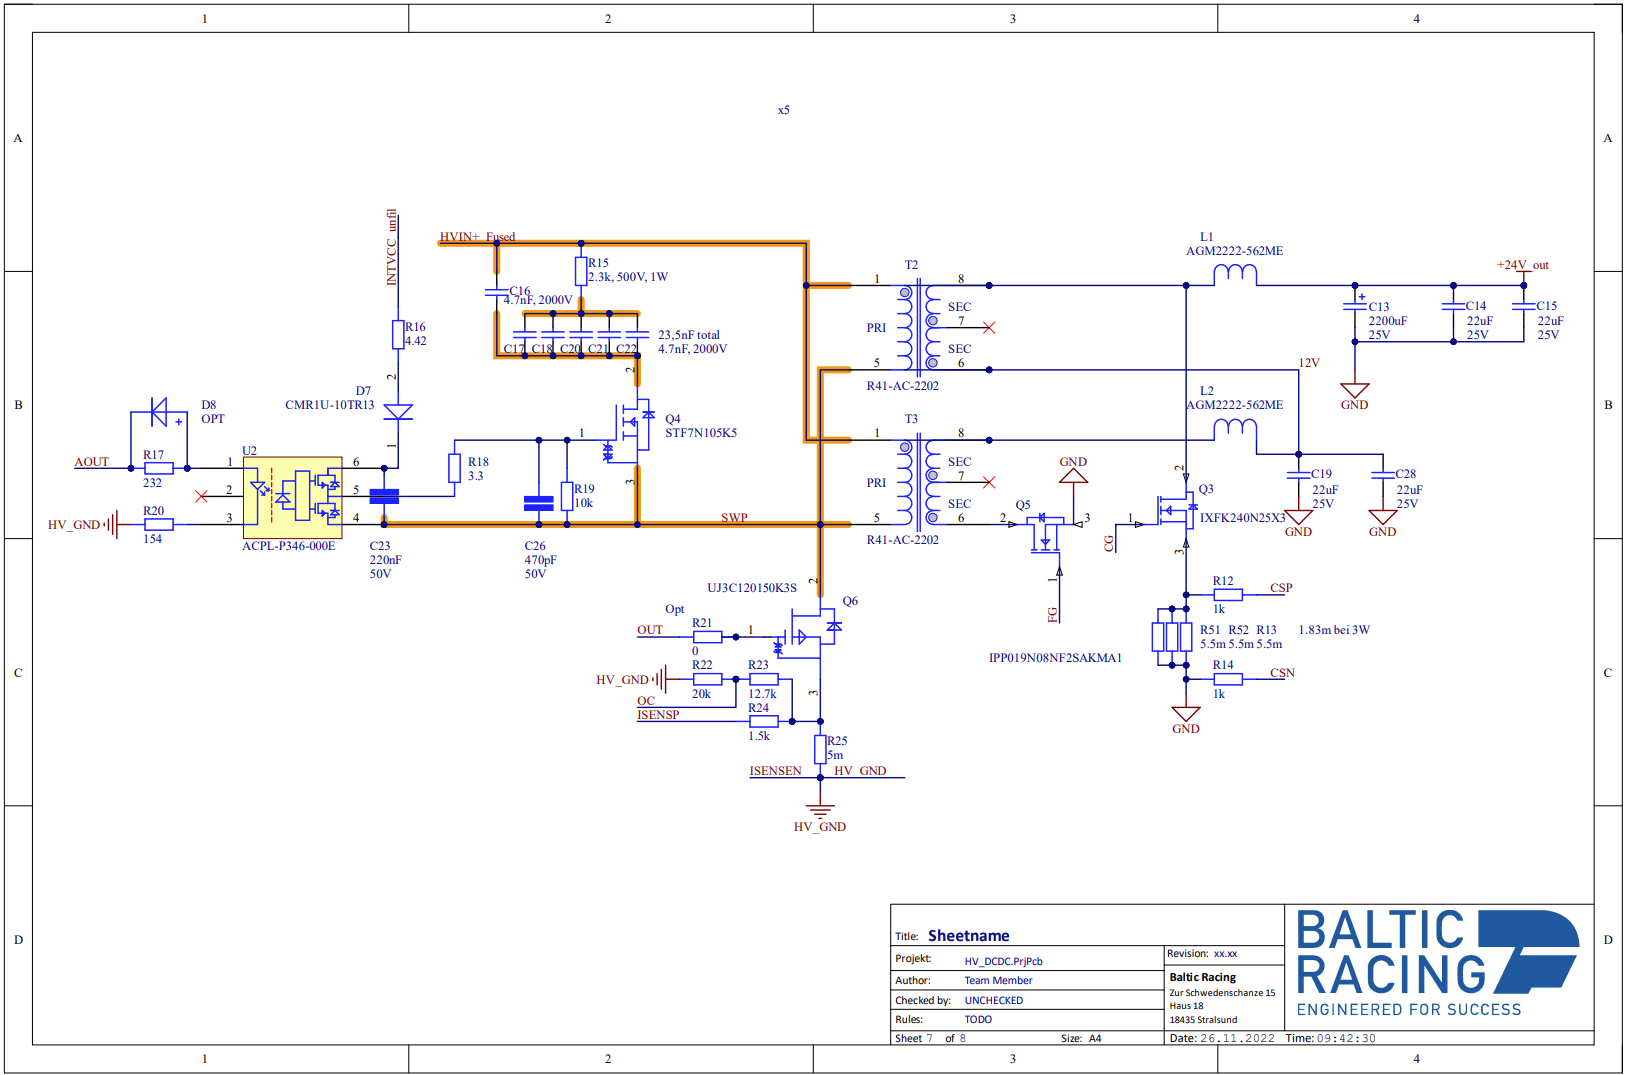
\includegraphics[width=1\linewidth]{bilder/HVDCDC_Transformer_Schematic}
	\caption{Schaltplan \ac{HV}-DCDC Transformer}
	\label{fig:hvdcdctransformerschematic}
\end{figure}

\FloatBarrier
\section{\ac{HV}-Distribution}
Bei der \ac{HV}-Distribution handelt es sich um eine Box welche mittig hinter dem Fahrer angeordnet ist. Diese Box beinhaltet alles an \ac{HV}-Elektrik was nicht im Akkumulator oder in den Umrichtern zu finden ist. Hier ist auch der \acfirst{HVD} untergebracht.

\FloatBarrier
\subsection{\ac{TSMP}}
Die \acfirst{TSMP} befinden sich seitlich am Fahrzeug wo auch der Hauptschalter zu finden ist. Sie stellen eine genormte Schnittstelle dar um mit einem Duspol, oder Multimeter an die Spannung des \ac{TS} gelangen zu können. Hierbei müssen laut Regelwerk \cite{FSRules} geschirmte Bananenstecker eingesetzt werden. Weiter muss für die Buchsen am Fahrzeug eine Abdeckkappe oder Blindstecker vorgesehen werden. Zur Absicherung der \ac{TSMP} müssen diese mit Widerständen in Reihe an den \ac{HV}-Kreis angebunden werden. Das Regelwerk sieht hierbei in unserem Spannungsbereich \ensuremath{15k\Omega} vor. Der Kritische Wert wonach die \ac{TSMP} ausgelegt werden müssen ist das Leistungsrating, da diese auf kontinuierlichen Kurzschluss ausgelegt sein müssen.
\\
\\
Eine Formel zu Berechnung der Leistung am Widerstand ist folgende.

\begin{equation}
	\label{eqn:Leistung am Wiederstand}
	\glsc{symb:P_elektrisch} = \glsc{symb:I}^{2} * \glsc{symb:R}
\end{equation}

Der Strom errechnet sich aus.

\begin{equation}
	\label{eqn:URI}
	\glsc{symb:U} = \glsc{symb:R} * \glsc{symb:I}
\end{equation}

Umgestellt nach I.

\begin{equation}
	\label{eqn:IUR}
	\glsc{symb:I} = \dfrac{\glsc{symb:U}} {\glsc{symb:R}}
\end{equation}

Da im Kurzschlussfall die Spannung über beide Widerstände anliegt, verdoppelt sich der Widerstand.

\begin{table}[h]
	\centering
	\caption{\ac{TSMP} Berechnung}
	\begin{tabular}{|c|c|c|}
		\hline
		\multicolumn{3}{|c|}{Eingangsparameter} \\
		\hline
		\glsc{symb:R} & 15 & \ensuremath{k\Omega} \\
		\hline
		\glsc{symb:U} & 600 & \ensuremath{V} \\
		\hline
		\multicolumn{3}{|c|}{Ergebnisse} \\
		\hline
		\glsc{symb:I} & 20 & \ensuremath{mA} \\
		\hline
		\glsc{symb:P_elektrisch} & 12 & \ensuremath{W} \\
		\hline
	\end{tabular}
\end{table}

Daraus schlussfolgert sich das die \ensuremath{15k\Omega} Widerstände mindestens ein Leistungsrating von \ensuremath{12 W} benötigen.

\FloatBarrier
\subsection{\ac{BSPD}}

\begin{figure}
	\centering
	\includegraphics[width=0.6\linewidth]{"bilder/BSPD Blockdiagramm"}
	\caption{BSPD Blockdiagramm}
	\label{fig:bspd-blockdiagramm}
\end{figure}

Die Aufgabe des \acfirst{BSPD} ist es das Fahrzeug in dem Fall einer Störung des Gaspedales in einen sicheren Zustand zu überführen. Hierfür wird der Strom zu den Umrichtern als auch der Bremsdruck gemessen und beim Eintreten eines im Regelwerk definierten Schwellwertes für das gleichzeitige auftreten beider Signale muss das Abschalten des Antriebes erfolgen. Das Blockdiagramm \ref{fig:bspd-blockdiagramm} soll einen Überblick über den Signalfluss ermöglichen.\\
\\
Bei den Eingangsignalen handelt es sich um analoge Spannungen. Für Signalaufbereitung oder auch Digitalisierung der Signale werden Schmitt-Trigger eingesetzt. Die Logik besteht aus diversen Logikgattern und die Set-/Reset-Schaltung besteht aus RC-Gliedern mit nachgeschalteten Schmitt-Triggern. Beim \ac{SDC} handelt es sich um ein \acfirst{SSR} welches von der \ac{BSPD}-Logik schlussendlich angesteuert werden soll. Ein öffnen des \ac{SDC} führt damit zu einem Herunterfahren des Antriebes.\\
\\
Zur Auslegung von Schmitt-Triggern.
\begin{figure}
	\centering
	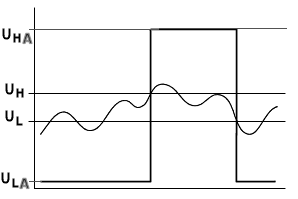
\includegraphics[width=0.4\linewidth]{bilder/Schmitt-trigger-diagramm.png}
	\caption{Signal am Schmitt-Trigger \cite{SchmittTriggerMikrocontrollernet}}
	\label{fig:schmitt-trigger-diagramm}
\end{figure}

Die Funktionsweise eines Schmitt-Trigger kann anhand der Abbildung \ref{fig:schmitt-trigger-diagramm} erkannt werden. Er ermöglicht es ein analoges Signal in ein Digitales umzuwandeln. Dabei ist es möglich festzulegen welche Spannungspegel am Ausgang des Schmitt-Trigger anliegen (\glsc{symb:U_HA} und \glsc{symb:U_LA}) bei welchen Spannungspegeln der Trigger high respektive low schalten soll (\glsc{symb:U_H} und \glsc{symb:U_L}). Das vorliegen unterschiedlicher Pegel zum Schalten wird Hysterese genannt. Sinn für das vorliegen ist, das Verhindern des rapiden Umschaltens zwischen den high und low Zuständen direkt am Schwellwert aufgrund von Signalrauschen.

\begin{figure}
	\centering
	\includegraphics[width=0.6\linewidth]{"bilder/TPS Failure detection"}
	\caption{Schaltplan Stromsignal Konditionierung}
	\label{fig:tps-failure-detection}
\end{figure}

\begin{figure}
	\centering
	\includegraphics[width=0.4\linewidth]{"bilder/nichtinvertierender Trigger"}
	\caption{Topologie des nicht Invertierenden Schmitt-Trigger \cite{SchmittTriggerMikrocontrollernet}}
	\label{fig:nichtinvertierender-trigger}
\end{figure}

Folgend Beispielhaft die Auslegung eines nicht Invertierenden Schmitt-Triggers wie er in der Abbildung \ref{fig:nichtinvertierender-trigger} zu sehen ist. Die andere Ausführung ist die eines Invertierenden.
\\
\\
Zur Berechnung sollten sich \glsc{symb:U_HA} und \glsc{symb:U_LA} sowie \glsc{symb:U_H} und \glsc{symb:U_L} aus dem Betriebsfall ergeben. R\textsubscript{1} sowie R\textsubscript{3} können frei gewählt werden. R\textsubscript{1} ist hierbei der Verbund aus R\textsubscript{3} und R\textsubscript{4}.
\\
\\
Die beiden folgenden Gleichung liegen zu Grunde.

\begin{equation}
	\label{eqn:Obere Hysteresespannung Schmitt Trigger}
	\glsc{symb:U_H} = \glsc{symb:U_ref} + (\glsc{symb:U_HA} - \glsc{symb:U_ref}) * \dfrac{R\textsubscript{1}} {R\textsubscript{1}+R\textsubscript{2}}
	mit R\textsubscript{1}=\dfrac{R\textsubscript{3}*R\textsubscript{4}}{R\textsubscript{3}+R\textsubscript{4}}
\end{equation}

Und

\begin{equation}
	\label{eqn:Untere Hysteresespannung Schmitt Trigger}
	\glsc{symb:U_L}=\glsc{symb:U_ref}-(\glsc{symb:U_ref}-\glsc{symb:U_HA})*\dfrac{R\textsubscript{1}}{R\textsubscript{1}+R\textsubscript{2}}
\end{equation}

Mit den folgenden Gleichungen lassen sich R\textsubscript{2} und R\textsubscript{4} bestimmen.

\begin{equation}
	\label{eqn:Berechnung R2 Schmitt Trigger}
	R\textsubscript{2} = R\textsubscript{1} * \dfrac{\glsc{symb:U_HA} - \glsc{symb:U_LA}} {\glsc{symb:U_H} - \glsc{symb:U_L}}
\end{equation}

\begin{equation}
	\label{eqn:Berechnung Uref Schmitt Trigger}
	\glsc{symb:U_ref} = (\glsc{symb:U_H} - \glsc{symb:U_LA}) * \dfrac{R\textsubscript{2}} {R\textsubscript{1} + R\textsubscript{2}} + \glsc{symb:U_LA}
\end{equation}

\begin{equation}
	\label{eqn:Berechnung R4 Schmitt Trigger}
	R\textsubscript{4} = R\textsubscript{3} * \dfrac{\glsc{symb:VCC}-\glsc{symb:U_ref}} {\glsc{symb:U_ref}}
\end{equation}

\begin{figure}
	\centering
	\includegraphics[width=0.6\linewidth]{"bilder/BSPD Integrator"}
	\caption{Schaltplan \ac{BSPD}-Integrator}
	\label{fig:bspd-integrator}
\end{figure}

Die Zeitsteuerung besteht aus einem Kondensator C2 welcher über den Widerstand R20 geladen wird, einer Diode D3 um Rückkopplung zu vermeiden, einem Widerstand R23 um den Kondensator langsam zu entladen, einem Spannungsfolger OP2 um die Schaltung von dem nachgeschalteten Schmitt-Trigger zu entkoppeln und einem Transistor T3 der den Kondensator in kurzer Zeit bei Bedarf entladen kann.\\
\\
Für die Berechnung ist die Ladezeit des Kondensators über den Widerstand R20 bis zur Schaltspannung des Schmitt Triggers zu ermitteln. Dies lässt sich mit folgender Gleichung Lösen. 

\begin{equation}
	\label{eqn:Ladezeit Kondensator}
	\glsc{symb:U_a}=\glsc{symb:U_e}*(1-\glsc{symb:e}^{\dfrac{1}{\glsc{symb:R}*\glsc{symb:C}}*\glsc{symb:t}})
\end{equation}

Alternativ kann der Schmitt-Trigger aber auch auf das 0,63 fache der Eingangsspannung gesetzt werden was der einfachen Zeitkonstante des RC Gliedes entspricht. Damit bestimmt sich C wie folgt.

\begin{equation}
	\label{eqn:Zeitkonstante Kondensator}
	\glsc{symb:C}=\dfrac{\glsc{symb:tau}}{\glsc{symb:R}}
\end{equation}

Mit Beispielhaften Auslegeparametern ergeben sich folgende Werte.

\begin{table}[h]
	\centering
	\caption{Schmitt-Trigger Rechnung}
	\begin{tabular}{|c|c|c|}
		\hline
		\multicolumn{3}{|c|}{Eingangsparameter} \\
		\hline
		\glsc{symb:tau} & 0,5 & \ensuremath{s} \\
		\hline
		\glsc{symb:R} & 100 & \ensuremath{k\Omega} \\
		\hline
		\multicolumn{3}{|c|}{Ergebnisse} \\
		\hline
		\glsc{symb:C} & 5 & \ensuremath{uF} \\
		\hline
	\end{tabular}
\end{table}

Das  \ac{BSPD}-Sensorboard hat zum Zweck einen Stromsensor zu kreieren der ein Stromsignal von \ensuremath{0-100 A} in ein Spannungssignal von \ensuremath{0,5-4,5 V} über den Bereich von \ensuremath{0-10 A} umwandelt. Die \ensuremath{0.5 V} Offset haben zum Ziel eine Kurzschlusserkennung auf Masse als auch auf Versorgung zu ermöglichen. Der relevante Messbereich von \ensuremath{0-10 A} entsteht aus den Regelwerksanforderungen die vorgeben das der Fehlerzustand bei einer abgerufenen Leistung größer 5kW eingestellt werden muss, was bei \ensuremath{600 V} in einem Strom von \ensuremath{8,3 A} resultiert. Dieser Bereich muss möglichst robust ausgewertet werden können.
\\
\\
Zur genauen Funktion. U1 ist ein Hall-Effekt Stromsensor der Firma Vakuumschmelze mit einem Übersetzungsfaktor von 1000 \cite{T60404-N4646-X100}. Heißt \ensuremath{10 A} ergeben \ensuremath{10 mA} Stromfluss am Ausgang. Der Widerstand R2 ist so gewählt das bei einem Strom von \ensuremath{10 mA}, \ensuremath{5 V} über den Widerstand abfallen und wir so in den Messbereich kommen. Der Widerstand R1 ermöglicht nun das konstante einspeisen von ca. \ensuremath{0,5 V} und die Diode das Begrenzen der max. Spannung auf \ensuremath{4,5 V}.

\begin{figure}
	\centering
	\includegraphics[width=0.7\linewidth]{"bilder/Sensorboard Schaltung"}
	\caption{Schaltplan \ac{BSPD}-Sensorboard}
	\label{fig:sensorboard-schaltung}
\end{figure}

\FloatBarrier
\subsection{Discharge}
Die Discharge Schaltung soll bei Abschalten des Fahrzeug die Zwischenkreiskondensatoren entladen. Ziel ist es das System möglichst schnell in einen Spannungsfreien und damit sicheren Zustand zu überführen.
\begin{figure}
	\centering
	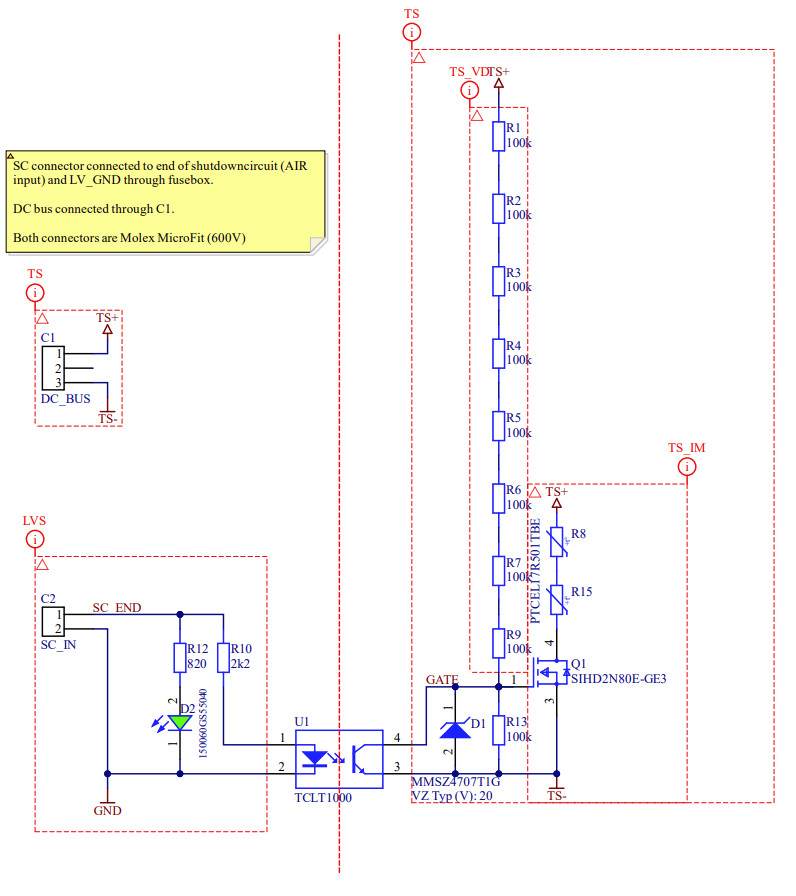
\includegraphics[width=0.8\linewidth]{bilder/Discharge}
	\caption{Schaltplan Discharge}
	\label{fig:discharge}
\end{figure}

Dies kann mit Hilfe von \ac{PTC}-Widerständen geschehen. Das Regelwerk sieht vor das der Zwischenkreis in maximal \ensuremath{5 s} auf \ensuremath{60 V\ac{DC}} oder weniger zu bringen ist. Dies muss für 3 aufeinanderfolgende Entladevorgänge möglich sein. 
\\
\\
Die Ansteuerung erfolgt über den \ac{SDC} welcher über den Steckverbinder C2 eingebunden ist. Von dort wird der Optokoppler U1 bestromt. Dieser steuert Strom vom Gate des Mosfet`s Q1 weg Richtung \ac{TS}- so das der Mosfet öffnet. Wenn der \ac{SDC} geöffnet wird, steigt die Spannung am Gate auf \ensuremath{20 V} und der Mosfet steuert \ac{TS}+ auf \ac{TS}- über die \ac{PTC}-Widerstände durch. Dadurch wird die Spannung im Zwischenkreis in den \ac{PTC}-Elementen abgebaut.
\\
\\
Die Formel für die Berechnung der \ac{PTC}-Elemente ist dem Datenblatt \cite{PTCManual} zu entnehmen.

\begin{equation}
	\label{eqn:PTC Berechnung}
	\glsc{symb:N_PTC}=\dfrac{\glsc{symb:N_dump} * \glsc{symb:K} * \glsc{symb:C} * \glsc{symb:U}^{2}} {2 * \glsc{symb:R} * \glsc{symb:C_th} * (\glsc{symb:T_SW} - \glsc{symb:T_u})}
\end{equation}

\begin{table}[h]
	\centering
	\caption{\ac{PTC} Berechnung}
	\label{PTC Berechnung}
	\begin{tabular}{|c|c|c|c|}
		\hline
		\multicolumn{4}{|c|}{Eingangsparameter} \\
		\hline
		\glsc{symb:T_SW} & 130 & \ensuremath{^\circ C} & Datenblatt Wiederstandsverlauf \\
		\hline
		\glsc{symb:K} & 1 & \ensuremath{-} & Datenblatt -> DC \\
		\hline
		\glsc{symb:C_th} & 2,3 & \ensuremath{J/K} & Datenblatt -> PTCEL17 \\
		\hline
		\glsc{symb:T_u} & 60 & \ensuremath{^\circ C} & Worst Case \\
		\hline
		\glsc{symb:C} & 400 & \ensuremath{uF} & 2x DTI 500 Kapazität \\
		\hline
		\glsc{symb:U} & 600 & \ensuremath{V} & \\
		\hline
		\glsc{symb:N_dump} & 4 & \ensuremath{-} & min 3 Regelwerk\\
		\hline
		\multicolumn{4}{|c|}{Ergebnisse} \\
		\hline
		\glsc{symb:N_PTC} & 1,79 & \ensuremath{-} &  \\
		\hline
	\end{tabular}
\end{table}

Mit den Ergebnissen aus Tabelle \ref{PTC Berechnung} ergibt sich das 2 \ac{PTC}`s des Typ 17R251 oder 17R501 verwendet werden müssen. 
\\
\\
Die Entladezeit kann wie beim \ac{BSPD} über die Zeitkonstante bestimmt werden, in diesem Fall näherungsweise über die 3 fache, da \ensuremath{3\tau = 95\%}Entladung und \ensuremath{600V\ac{DC} * 0,05 = 30V\ac{DC}} Damit ergibt sich eine Entladezeit von max. \ensuremath{1,2 s}.

\FloatBarrier
\section{\ac{TSAL}}
Das \acfirst{TSAL} ist eine Lampe am Mainhoop die 360 Grad rundherum zum Fahrzeug anzeigt ob das \ac{TS} eingeschaltet ist oder nicht und ob ein Fehler vorliegt. Damit ergeben sich drei Zustände, \ac{TSAL} Rot blinkend heißt \ac{TS}-on, \ac{TSAL} grün leuchtend heißt \ac{TS}-off und \ac{TSAL} aus heißt entweder \acfirst{LVS} ausgeschaltet oder Fehler im \ac{TS}. Die gesamte Logik ist dabei in nicht programmierbaren Bausteinen umzusetzen.

\FloatBarrier
\subsection{Logik auf Discharge}
\label{sec: TSAL Logik Discharge}
\begin{figure}
	\centering
	\includegraphics[width=0.9\linewidth]{"bilder/Binäre Spannungserkennung"}
	\caption{Schaltplan Konstantstromquelle Discharge}
	\label{fig:binare-spannungserkennung}
\end{figure}

Das Herz der Schaltung ist ein Verarmungstyp N-Fet \cite{IXTA08N100D2HV}. Wenn die Gate-Source Spannung V\textsubscript{GS} = \ensuremath{0 V} ist, dann lässt dieser Fet Strom durch. Ab einer Spannung von \ensuremath{47 V} wird die Zehnerdiode durchbrochen und ein Strom fließt, dieser Strom verursacht einen Spannungsabfall am Widerstand R18 von ca. \ensuremath{2,2 V} bei einem \ensuremath{mA} so das V\textsubscript{GS} negativ wird und der Fet den Stromfluss zu begrenzen beginnt. Der Fet agiert zusammen mit dem Widerstand wie eine Konstantstromquelle. Diese Steuert den Optokoppler durch so das wir auf der \acfirst{LV}-Seite ein Signal erzeugt haben.

\FloatBarrier
\subsection{Logik auf \ac{AMS} Master}

Nachdem die diversen Signale für den Zustand der \ac{AIR}`s etc. vorliegen geht es darum sie logisch miteinander zu verschalten. Zuerst wird dafür in U8\textsubscript{a-c} verglichen ob die vorhergesehen und tatsächlichen Zustände für die Relais übereinstimmen. Die XOR-Gatter geben dabei immer einen High-Pegel und damit einen Fehlerzustand aus, wenn dies nicht der Fall ist. Zweitens gilt es nun zu plausibilisieren ob auch Spannung auf dem System anliegt. Sofern entweder der Precharge oder das positive \ac{AIR} und das negative \ac{AIR} geschlossen ist bedeutet dies, dass der Stromkreis geschlossen ist. Damit sollte Spannung anliegen. Da die Relais Signale bereits plausibilisiert wurden geht es bei dieser Schaltung darum zu prüfen ob das Spannungssignal etwas anzeigt, wenn dies vom Relais Zustand her der Fall sein sollte. Der Fehlerzustand tritt in der Schaltung nur ein wenn die Ausgänge von U11A und U12A high sind, was wiederum dadurch hervorgerufen wird, das bei U11A das Signal vom Precharge oder das vom positiven \ac{AIR} high ist und bei U12A das Signal vom negativen \ac{AIR} high ist und das Danger-V-Signal low ist. Anschließend werden all diese Signale noch mit dem \ac{AIR}-error-Ausgang verodert und in den Latch gegeben. Der Latch besteht hauptsächlich aus dem FlipFlop U26\textsubscript{A}. Der Sinn dieses ist, das wenn ein Fehler gesetzt wird dieser auch permanent bestehen bleibt und das System sich nicht selbst zurücksetzten kann. Um beim Einschalten des Systems unplausible Zustände abzufangen befindet sich ein RC-Glied am CLR-Eingang des FlipFlop so das dieser solange keine Signale annimmt bis das System den stationären Zustand erreicht hat. Nun gibt es noch an U9\textsubscript{B} das \ac{TS}-ON Signal welches eine veroderung der verschiedenen Relais- und des Spannungs/-Signales darstellt. Heißt wenn irgendwas mit den \ac{AIR}`s passiert oder Spannung auf dem System liegt ist das \ac{TS}-on. Der Ausgang des Error Latches und des \ac{TS}-on Signales wird nun in ein NOR-Gatter gegeben so das der GRN-ON Zustand der das \ac{TSAL} grün aufleuchten lässt nur eintritt wenn was \ac{TS} nicht on ist und kein Fehler vorliegt. Weiter ist das Signal noch mit dem \ac{POR} verundet so, dass das Grün-Signal erst aufleuchtet wenn das System auch tatsächlich arbeitet.

\begin{figure}
	\centering
	\includegraphics[width=1\linewidth]{"bilder/TSAL Logik AMS Master"}
	\caption{Schaltplan \ac{TSAL}-Logik \ac{AMS}-Master}
	\label{fig:tsal-logik-ams-master}
\end{figure}

\FloatBarrier
\subsection{Schaltung auf \ac{TSAL}}

Das \ac{TSAL} besteht wesentlich aus drei funktionellen Blöcken. Der Blink-Schaltkreis basierend auf einem NE 555, Die \ac{LED}`s selber und ein \ac{LED}-Treiber mit seiner Beschaltung. Der \ac{LED}-Treiber ist nach Datenblatt aufgebaut. Das Red- und das Green-/Signal gehen beide auf den \ac{PWM}-Eingang des Treibers so das wenn das \ac{TSAL} aus sein soll der Treiber in den sleep mode geht. Bei den \ac{LED}`s handelt es sich um Horticulture 6868 Ceramic \ac{LED}`s von \ac{WE}. Diese wurden in den vorherigen Jahren auch auf dem Bremslicht verwendet und zeichnen sich durch hohe Leistungsdichte aus. Am Ende der \ac{LED}-Ketten befindet sich ein Mosfet welcher durch das Red oder Green Signal durchgeschaltet und damit der Stromkreis um die \ac{LED}`s geschlossen wird. Der NE 555 wird genutzt um ein Taktsignal mit einer Frequenz von \ensuremath{2-5 Hz} zu erzeugen. Dies wird benötigt da das \ac{TSAL} im Falle des eingeschalteten \ac{TS} mit einer Frequenz in diesem Bereich rot blinken soll.

\begin{figure}
	\centering
	\includegraphics[width=1\linewidth]{"bilder/Tsal Schematic"}
	\caption{Schaltplan \ac{TSAL}}
	\label{fig:tsal-schematic}
\end{figure}

\FloatBarrier